% -------------------------------------------------------------------- %
% -------------------------------------------------------------------- %
% -------------------------------------------------------------------- %

\documentclass[twocolumn,10pt,dvipsnames]{article} % here we use the article class, rather than elsarticle

% -------------------------------------------------------------------- %
% -------------------------------------------------------------------- %
% -------------------------------------------------------------------- %

\usepackage[square,numbers,sort&compress,comma]{natbib}

\usepackage{amsmath}
\usepackage{amssymb}
\usepackage{caption}
\usepackage{graphicx}
\usepackage{latexsym}
\usepackage{times}
\usepackage[pagewise]{lineno}
\usepackage{chemmacros}
\usepackage{chemfig}
\usepackage{chemformula}
\usepackage{siunitx}
% \usepackage[dvipsnames]{xcolor}

% -------------------------------------------------------------------- %
% -------------------------------------------------------------------- %
% -------------------------------------------------------------------- %

\topmargin - 12pt % might need to be set to 0pt for some installations
\oddsidemargin 32pt
\textheight 610pt
\textwidth 408pt
\columnsep 24pt

\newcommand{\mrm}[1]{\mathrm{#1}}
\newcommand{\rmd}{\mrm{d}}
\newcommand{\rme}{\mrm{e}}
\newcommand{\rmf}{\mrm{f}}
\newcommand{\rmm}{\mrm{m}}
\newcommand{\rmp}{\mrm{p}}
\newcommand{\rmr}{\mrm{r}}
\newcommand{\rms}{\mrm{s}}
\newcommand{\Ru}{R_\mrm{u}}

\newcommand{\upd}{\mathrm{d}}                           % Upright d as derivative operator
\newcommand{\upe}{\mathrm{e}}                           % Upright e as mathematical constant
\newcommand{\der}[2]{\frac{\upd #1}{\upd #2}}           % Derivative
\newcommand{\pder}[2]{\frac{\partial #1}{\partial #2}}  % Partial derivative
\newcommand{\bvec}[1]{{\bm{{#1}}}}                      % Vector (bold italic)

\chemsetup{
  formula = mhchem ,
  modules  = {reactions}
}

% -------------------------------------------------------------------- %
% -------------------------------------------------------------------- %
% -------------------------------------------------------------------- %

\def\thepage{}

\renewenvironment{abstract}%
              {% - begin definition
               \small% - select font
               {\bfseries \abstractname}% - select font
               \par% - end a paragraph (skip \parsep)
               \vspace{10pt}% - add vertical space
              }% - complete definition

\renewcommand\abstractname{Abstract}

\newcommand{\nomenclature}% - name of command
              [1]% - number of arguments
              {% - begin definition
               \bgroup% - begin a local group
               \flushleft% - turn on flushleft option
               \small\bf% - select font
               #1% - insert title text
               \par% - end a paragraph (skip \parsep)
               \egroup% - terminate local group
              }% - complete definition

\renewcommand{\section}% - name of command
              [1]% - number of arguments
              {% - begin definition
               \bgroup% - begin a local group
               \flushleft% - turn on flushleft option
               \small\bf% - select font
               \refstepcounter{section}% - increment counter
               \arabic{section}. #1% - insert title text
               \par% - end a paragraph (skip \parsep)
               \egroup% - terminate local group
              }% - complete definition

\renewcommand{\subsection}% - name of command
              [1]% - number of arguments
              {% - begin definition
               \bgroup% - begin a local group
               \flushleft% - turn on flushleft option
               \small\em% - select font
               \refstepcounter{subsection}% - increment counter
               \arabic{section}.% - insert title text
               \arabic{subsection}. #1% - insert title text
               \par% - end a paragraph (skip \parsep)
               \egroup% - terminate local group
              }% - complete definition

\renewcommand{\subsubsection}% - name of command
              [1]% - number of arguments
              {% - begin definition
               \bgroup% - begin a local group
               \flushleft% - turn on flushleft option
               \small\em% - select font
               \refstepcounter{subsubsection}% - increment counter
               \arabic{section}.% - insert title text
               \arabic{subsection}.% - insert title text
               \arabic{subsubsection}. #1% - insert title text
               \par% - end a paragraph (skip \parsep)
               \egroup% - terminate local group
              }% - complete definition

  \newcommand{\acknowledgement}% - name of command
              [1]% - number of arguments
              {% - begin definition
               \bgroup% - begin a local group
               \flushleft% - turn on flushleft option
               \small\bf% - select font
               #1% - insert title text
               \par% - end a paragraph (skip \parsep)
               \egroup% - terminate local group
              }% - complete definition

  \newcommand{\sectionbib}% - name of command
              [1]% - number of arguments
              {% - begin definition
               \bgroup% - begin a local group
               \flushleft% - turn on flushleft option
               \small\bf% - select font
               #1% - insert title text
               \par% - end a paragraph (skip \parsep)
               \egroup% - terminate local group
              }% - complete definition

\renewcommand\figurename{Fig.}
\renewcommand{\captionsize}{\footnotesize}
\setlength\abovecaptionskip{0pt}
\setlength\belowcaptionskip{0pt}

\renewcommand\bibsection{\sectionbib{\refname}}

\setlength\bibsep{0pt}

\pagenumbering{arabic}

\newcommand{\red}{\color{red}}
\newcommand{\blue}{\color{blue}}
\newcommand{\green}{\color{ForestGreen}}
\newcommand{\orange}{\color{orange}}
\newcommand{\pink}{\color{Salmon}}

% \newcommand{\red}{}
% \newcommand{\blue}{}
% \newcommand{\green}{}
% \newcommand{\orange}{}
% \newcommand{\pink}{}



% -------------------------------------------------------------------- %
% -------------------------------------------------------------------- %
% -------------------------------------------------------------------- %

\begin{document}

\title{\LARGE \green Numerical study probing the effects of preferential concentration on the combustion of iron particles in a mixing layer}

\author{{\large Shyam Hemamalini$^{a,b}$, B\'en\'edicte Cuenot$^{a,c}$, Jeroen van Oijen$^{a}$, \\XiaoCheng Mi$^{a,b,*}$}\\[10pt]
        {\footnotesize \em $^a$Department of Mechanical Engineering, Eindhoven University of Technology\\[-5pt]
        \footnotesize \em P.O. Box 513, 5600MB, Eindhoven, The Netherlands}\\
        {\footnotesize \em $^b$Eindhoven Institute of Renewable Energy Systems, Eindhoven University of Technology\\[-5pt]
        \footnotesize \em P.O. Box 513, 5600MB, Eindhoven, The Netherlands}\\
        {\footnotesize \em $^c$CERFACS\\[-5pt] \footnotesize \em 42, Avenue G. Coriolis, 31057 Toulouse Cedex 01, France}\\
        {\footnotesize $^*$ Corresponding author}}

\date{}

% -------------------------------------------------------------------- %
% -------------------------------------------------------------------- %
% -------------------------------------------------------------------- %

\small
\baselineskip 10pt

% -------------------------------------------------------------------- %
% -------------------------------------------------------------------- %
% -------------------------------------------------------------------- %

\twocolumn[\begin{@twocolumnfalse}
\vspace{50pt}
\maketitle
\vspace{40pt}
\rule{\textwidth}{0.5pt}
\begin{abstract} % 100 to 300 words.
%
The iron power cycle is a novel carbon-free energy storage technology that has seen considerable advancement over the past few years. The design of large-scale industrial iron powder combustors relies on a good understanding of not only the combustion process of $\mrm{Fe}$ particles but also the interaction of the burning particles with complex turbulent flow structures. Preferential concentration is one such effect observed in turbulent particle-laden flows, that clusters particles into regions of high particle concentrations. To simulate such phenomena of particle-flow interactions for reacting $\mrm{Fe}$ particles, we first establish a numerical framework based on a coupled Eulerian-Lagrangian approach and a switch-type $\mrm{Fe}$ combustion model. A mixing layer is chosen as the canonical flow scenario to simulate particle-flow interactions. In the present work, the effects of preferential concentration on different particle sizes $d_\mrm{p} = \left( 14,20,28,39,55 \right)\SI{}{\micro\meter}$ are captured and examined. The smaller particles with $d_\mrm{p} \leq \SI{20}{\micro\meter}$ retain the structure of the mixing layer whereas the larger particles $d_\mrm{p} \geq \SI{28}{\micro\meter}$ perturb the mixing layer and significantly alter the imposed flow structure. In the present work, we use minimum spacing $\delta_\mrm{min}$, normalized by the mean interparticle distance $\bar{\delta}$, to quantify particle clustering through preferential concentration. In the cases with sufficiently larger particles ($d_\mrm{p} \geq \SI{28}{\micro\meter}$), particles with longer burn times $\tau_\mrm{B}$ statistically exhibit lower values of minimum spacing, indicating particle clustering which results in the localized depletion of $\mrm{O_2}$. {\pink A comparison of minimum spacing with simulations of inert particles shows a deviation in the mean and mode of minimum spacing for $\SI{39}{\micro\meter}$ particles that coincide with the overall combustion burnout times. This deviation is attributed qualitatively to the modification of the particle relaxation and flow timescales as a consequence of particle combustion. Further analysis to quantify the timescales involved in Fe combustion might be beneficial in achieving deeper insight into this deviation.}
%
\end{abstract}
\vspace{10pt}
\parbox{1.0\textwidth}{\footnotesize {\em Keywords:} Metal fuels; Iron powder combustion; Heterogeneous combustion; Turbulent iron flames; Carbon-free renewable fuels}
\rule{\textwidth}{0.5pt}
\vspace{10pt}

\end{@twocolumnfalse}] 

\clearpage

\twocolumn[\begin{@twocolumnfalse}

\centerline{\bf Information for Colloquium Chairs and Cochairs, Editors, and Reviewers}

\vspace{20pt}
\iffalse
{\em
Note: The explanatory material in italic font on this page should be removed prior to manuscript submission.
\vspace{10pt}

On page 2 of their submission, authors are to provide three pieces of information:
1) a brief statement of the novelty and significance of the work reported in the manuscript;
2) a brief statement of each author's contributions to the manuscript;
and 3) the authors' preference and justification for the mode of presentation at the Symposium, in the event that the manuscript is accepted for presentation. The first two of these are consistent with current requirements for publication in Combustion and Flame and other journals. The third is specific to presentation at the Symposium. This material will not be included in the published paper, in the event that the manuscript is accepted for publication in the Proceedings.
}

\vspace{20pt}
\fi
{\bf 1) Novelty and Significance Statement}
\vspace{10pt}
\iffalse
{\em
A ``novelty and significance'' paragraph is required for all manuscripts. The minimum length is 50 words and the maximum 150 words. This paragraph should provide a concise statement for editors and reviewers to use in determining whether or not the contribution warrants acceptance for presentation at the Symposium and publication in the Proceedings.
}

\vspace{10pt}
\fi

In this research, we focus on modelling particle-flow interactions of reacting Fe particles in a turbulent flow. Such interactions have profound implications in the combustion process, and understanding these interactions is essential in the design of practical industrial-scale turbulent iron powder combustors. Hence, this research is very significant to the topic of iron powder combustion.

\vspace{10pt}

A novel numerical framework to model the flow-particle interactions is developed. The phenomenon of preferential concentration of reacting Fe particles is also novel to this field, as it involves the complex interplay of fluid dynamical phenomena and the non-volatile combustion of iron particles. This work is one of the pioneering efforts in the field of metal fuels and iron power research to focus on the interaction of reacting $\mrm{Fe}$ particles with turbulent flows. The effects of particle sizes (associated with different Stokes-number regimes) and energy release from combustion on the complex reactive particle-laden flow dynamics with preferential concentrations are investigated for the first time in literature.

\vspace{20pt} 

{\bf 2) Author Contributions}
\vspace{10pt}
\iffalse
{\em
The authors should be identified by their initials and each author's contributions to the manuscript should be indicated by 2-3 words such as, for example, ``designed research,'' ``performed research,'' ``analyzed data,'' ``wrote the paper,'' etc.
}
\fi
\begin{itemize}

  \item First author, SH, has designed, performed research, analyzed data and wrote the paper.

  \item Second author, BC, has designed research, provided feedback and interpreted results. BC has also proofread and presented feedback on manuscript.

  \item Third author, JO, has helped in procuring resources, and provided help in optimization of tools. JO has also proofread and presented feedback on manuscript.

  \item Fourth author, XM, has acquired funding, designed research, analysed data, and interpreted results. XM has also aided in the organization and revision of the manuscript.

\end{itemize}

\vspace{10pt}

{\bf 3) Authors' Preference and Justification for Mode of Presentation at the Symposium}
% \vspace{10pt} 
\iffalse
{\em
As discussed in the information provided to authors, two formats will be available for presentation of papers at the Symposium: Oral Presentation Papers (OPPs) and Poster Presentation Papers (PPPs). Here authors are to specify their preference for OPP or PPP presentation, and to justify their preference with 3-5 highlights ($<$120 characters each, spaces included). The highlights should be consistent with the criteria that are given in the Criteria to Differentiate document that is available to authors. This authors' preference and justification will be considered in the decision making, although there is no guarantee that the authors' preferred mode of presentation can be accommodated. The mode of presentation for papers accepted for presentation at the Symposium will have no bearing on the decision on whether or not the submission is accepted for publication in the Proceedings.
}
\fi
\vspace{10pt}

The authors prefer \textbf{OPP} presentation at the Symposium, for the following reasons:

\begin{itemize}

  \item The paper is deemed to have the potential of adding value to the community through a room-wide audience discussion. Flow-particle interactions are fundamental phenomena that affect the combustion process of $\mrm{Fe}$ particles.

  \item The research in this paper focuses on results that does not require prior context in the field of research this to which this paper contributes. The consequences of flow-particle interactions are well-known to the majority of researchers working in this topic.

  \item The approach used in this paper is novel compared to other research in the topic of metal fuels.

\end{itemize}

\end{@twocolumnfalse}] 

% -------------------------------------------------------------------- %
% -------------------------------------------------------------------- %
% -------------------------------------------------------------------- %

\clearpage

\linenumbers

\section{Introduction}
\label{sec:introduction}
\addvspace{10pt}

With the energy transition well underway, we have seen clean, green, carbon-free, renewable energy production techniques such as solar and wind energy gain substantial traction in scientific development over the past decade. The supply-demand mismatch caused by renewable energy sources like solar and wind energy has accelerated research in novel clean, carbon-free energy storage technologies such as hydrogen and lithium-ion batteries. The iron power cycle is one such novel renewable energy storage technology that has also seen considerable advancement over the latter part of the past decade.

\iffalse As a result of this advancement, a sizeable portion of the energy throughput of today consists of energy from such sources over the conventional coal and carbon-based energy forms of the past. Such energy sources bring unique problems of their own and the common among such natural renewable energy sources is the fluctuation in magnitude, time, and also geography. Considering solar energy -- which has been slowly domesticated and made available for use in household and industrial places alike -- as an example, the time of abundance of solar energy (daytime) is when we need energy the least. This mismatch in the energy supply and demand has turned the spotlight towards a part of the ecosystem -- energy storage. 

Over the past few years, research on energy storage has picked up pace. With the energy transition in mind, there has been significant research on clean, carbon-free energy sources such as hydrogen and lithium-ion batteries. \fi 

\iffalse 
There are countless studies that establish the advantages of the iron power cycle over both conventional-- hydrocarbons-- and modern-- hydrogen, lithium-ion batteries-- energy storage technologies. And like any innovative technology, the development of the iron power cycle and its practical use is not without obstacles. The purpose of the present study is to first establish a problem unique to the iron power cycle -- specifically the combustion process -- with the community, and next highlight the significance of said problem. 


\section{Problem Description}
\label{sec:description}
\addvspace{10pt}



The combustion of a single iron particle has been studied in great detail over the past few years by a few different groups. Ning et al. established benchmark experimental results for the combustion of a single iron particle. Panahi et al. conducted experiments at different oxygen concentrations and presented the temperature evolution of the burning particles. Whereas, Tang et al. and Li et al. established experimental results for an iron dust flame structure and propagation behavior. 

On the other hand, numerical modeling of the combustion process of a single iron particle has been established by Hazenberg and van Oijen and Mi et al. Recently, advanced single particle combustion models that incorporate complex phenomena such as evaporation of $\mathrm{Fe}$ and $\mathrm{FeO}$, Stefan flow, and higher oxidation states, have been put forward. 

\fi

The development of a large-scale iron powder combustor has also increased in pace with several industrial combustors in operation today. In such combustors, turbulent flow regimes are of utmost importance to ensure a sufficiently long residence time for the iron particles to be adequately oxidized \cite{Shoshyn2023}. Therefore, a good understanding of the complex interplay between reacting iron particles and turbulence is indispensable for the design of such large-scale combustors.

Preferential concentration is a phenomenon observed in turbulent particle-laden flows. It is described as the tendency of particles in a turbulent flow to inhomogenize, forming dense particle clusters and empty vortices. A comprehensive theoretical framework was established by Eaton and Fessler \cite{Eaton1994}, who highlight the significance of the Stokes number $\mrm{St}$ for the phenomenon. The Stokes number $\mrm{St}$ is defined as the ratio of the particle and the flow timescales, and Stokes numbers close to unity indicate strong, coupled particle-flow interactions.  

\begin{figure}[h!]
\centering
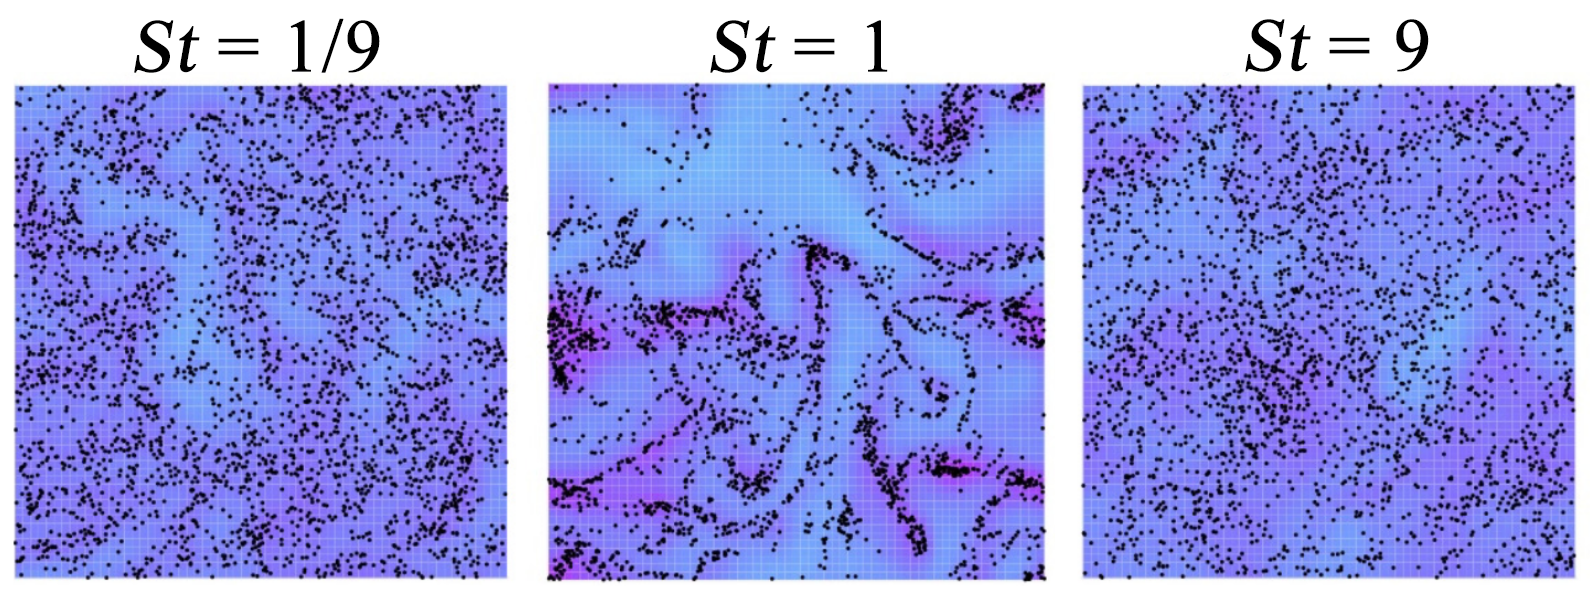
\includegraphics[width=172pt]{images/prefconc.png}
\caption{\footnotesize Example of preferential concentration seen when $\mrm{St} = 1$. Figure adapted from Pouransari and Mani \cite{pouransari2018}.}
\label{fig:prefconc}
\end{figure}

Iron is unique from other solid fuels such as magnesium, aluminum, and biomass in that it is non-volatile throughout the combustion process. The boiling point of iron (3134K) and iron oxide ($\mrm{FeO}$-3687K, $\mrm{Fe_3O_4}$-2896K) are sufficiently higher than the temperatures encountered in large-scale combustors, and hence, it is easy to conclude that iron particles--in their burnt or unburnt state--stay as solids or liquids and do not vaporize into the carrier phase (which is usually air). Thus, the presence of turbulence during the combustion process \emph{may} give rise to a preferential concentration of the burning $\mrm{Fe}$ particles, which has profound implications on the combustion process. For example, within regions of high particle concentrations, the local fuel equivalence ratio can be very high, leading to partial or total lack of ignition of some particles as a consequence of local depletion of $\mrm{O_2}$. {\green While there exists substantial literature on the physics of preferential concentration in particle-laden turbulence with inert particles, burning iron particles introduces a complexity that is insufficiently investigated in literature -- particle-laden turbulent reactive flows. Hence, the current study finds its purpose in initiating research in this topic.}

The primary objectives of this study are:
\begin{enumerate}
    \item To capture preferential concentration (or its absence) and quantify the magnitude of this phenomenon across different sizes of inert and reactive iron particles.
    \item To analyze the effect of the preferential concentration on the combustion process.
\end{enumerate}
Recently, Luu~et~al.~\cite{luu2024carrier} made the first attempt to investigate the ignition and combustion characteristics of $\SI{10}{\micro\meter}$-sized iron particles in a turbulent mixing layer driven by shear flows. This study reveals evidence showing that the oxidation rate of iron particles is hindered by local depletion of oxygen likely caused by preferential concentration. The current study finds its novelty in further probing the effects of varied particle sizes (associated with different Stokes-number regimes) and differences between scenarios with reactive and inert particles.

In Section 2\ref{sec:methodology}, we describe the numerical framework that was established to carry out DNS of reacting iron particles with sufficient complexity. In Section 3\ref{sec:simsetup}, a mixing layer is chosen as the canonical flow scenario to observe the clustering of iron particles. In this work, the effect of particle size on the preferential concentration is studied. Detailed description of the setup of the numerical simulations is also described in Section 3\ref{sec:simsetup}. Section 4 discusses the results from the simulations that were carried out, such as temperature contours, oxygen species mass fraction contours and burn time analyses to examine the effect of preferential concentration on the combustion process.

\section{Numerical Framework}\label{sec:methodology}\addvspace{10pt}

To model the interaction of the flow with the burning Fe particles, a numerical framework is developed based on an Eulerian-Lagrangian approach. 

\subsection{Gas-phase Model}\addvspace{10pt}
The gas phase is modeled using an Eulerian Cartesian grid and the compressible form of the Navier-Stokes equations of continuity, momentum, energy, and the species conservation equations are solved. Two-way coupling with the particle model is achieved by including the source terms from the particle model such as particle drag, heat transfer, and $\mrm{O_2}$ consumption. The gas-phase equations with the coupled particle-phase source terms read as:
\begin{equation}
    \frac{\partial \rho}{\partial t} + \frac{\partial \rho u_j}{\partial x_j} = S_\mrm{M}
\end{equation}
\begin{equation}
    \frac{\partial \rho u_i}{\partial t} + \frac{\partial \rho u_i u_j}{\partial x_j} = - \frac{\partial p}{\partial x_i} +  \frac{\partial \tau_{ij}}{\partial x_j} + S_\mrm{F,i}
\end{equation}
\begin{equation}
    \frac{\partial \rho e_t}{\partial t} + \frac{\partial (\rho e_t + p) u_j}{\partial x_j} =  \frac{\partial (u_j \tau_{ij})}{\partial x_i} -  \frac{\partial q_j}{\partial x_j} + S_\mrm{H}
\end{equation}
\begin{equation}
    \frac{\partial \rho Y_{\alpha}} {\partial t} + 
\frac{\partial \rho Y_{\alpha} u_j}{\partial x_j} 
= - \frac{\partial \rho Y_{\alpha} V_{\alpha j}} 
{\partial x_j} + S_\mrm{\alpha}
\end{equation}
\noindent where $S_\mrm{M}$, $S_\mrm{F,i}$, $S_\mrm{H}$ and $S_\mrm{\alpha}$ are the Lagrangian source terms of density, momentum, energy, and species mass fractions, respectively.
For this purpose, the high-order Fortran-based solver NTMIX-CHEMKIN \cite{poinsot1992boundary} is used. NTMIX-CHEMKIN is a highly-parallelized, spatially 8th-order, and temporally 3rd-order solver that has been used for solving subsonic reacting flows with good accuracy. {\red NTMIX-CHEMKIN has sufficient temporal resolution using the maximum acoustic signal speed ($\sim 1\mathrm{e}{-7}$s) which is sufficient for particle reaction kinetics.} It has been recently complemented with a Lagrangian solver for particle tracking. Thermophysical and chemical properties of the gas-phase species are computed using CHEMKIN. In our model, we do not account for any reactions in the gas-phase and hence, gas-phase chemistry is disabled. Trilinear interpolation is used to model the Lagrangian source terms at the location of each particle.

\subsection{Particle Model}\addvspace{10pt}
A heterogeneous combustion model framework \cite{Soo2018} is used since the flame temperature of iron flames and temperatures seen in practical combustors are lower than the boiling point of iron. Following this assumption, each iron particle is modeled with a point-source Lagrangian approximation that enables individual tracking of particles at all times on a virtually-infinitesimal grid.  The location $\mathbf{x}_{\mathrm{p}}$ and the velocity $\mathbf{u}_{\mathrm{p}}$ are tracked using the following set of equations:
\begin{equation}
\begin{split}
    \der{\mathbf{x}_{\mathrm{p}}}{t} &= \mathbf{u}_{\mathrm{p}}\\
    \der{\mathbf{u}_{\mathrm{p}}}{t} &= \frac{3}{4}\frac{C_\mrm{D} \rho}{d_\mathrm{p} \rho_\mathrm{p}}\left| \mathbf{u} - \mathbf{u}_{\mrm{p}} \right| \left( \mathbf{u} - \mathbf{u}_{\mathrm{p}} \right) 
\end{split}\label{eq:particledrag}
\end{equation}
\noindent where the subscript $\mrm{p}$ denotes particle properties. The particle acceleration constitutes the source term $S_\mrm{F,i}$ at the location of the respective particle in the gas-phase equations. The drag coefficient $C_D$ is calculated based on the Schiller-Naumann correlation:
\begin{equation}
    C_\mrm{D} = \frac{24}{\mathrm{Re}} (1+0.15\mathrm{Re}^{0.687})
\end{equation}

The specific heating value associated with the formation of $\mrm{FeO}$ is nearly 70\% of the maximum amount of heat that can be released by the liquid-phase iron oxidation with $\mrm{Fe_3O_4}$ as the end product. Since the mechanism of further oxidation beyond liquid $\mrm{FeO}$ is not yet well understood \cite{FujinawaAECS,ThijsCNF}, only the first step of iron oxidation is considered for simplicity:
\begin{reactions}
  2Fe + O2 -> 2FeO. \notag
\end{reactions}

The reaction model is similar to the switch-type model given by Mi et al. \cite{mi2022quantitative,jean2023ignition}, where the mass consumption of oxygen is determined as the slower one of the two rate-limiting processes-- solid-state diffusion of $\mathrm{Fe}$ ions through the $\mrm{FeO}$ layer and diffusion of $\mrm{O_2}$ from the bulk to the particle surface given by Eqs. \ref{eq:mr} and \ref{eq:diffo2}.
\begin{equation}
    \dot{m}_\mrm{FeO} = \frac{\rho_\mrm{FeO} A_\mrm{p} k_\mrm{0,FeO}}{X_\mrm{FeO}} \exp \left( \frac{-T_\mrm{a}}{T_\mrm{p}}\right) 
\end{equation}
\begin{equation}
    \dot{m}_\mrm{O_2,R} = \nu_\mrm{O_2/FeO}\ \dot{m}_\mrm{FeO} \label{eq:mr}
\end{equation}
\noindent where $A_\mrm{p}$ is the particle surface area, $T_\mrm{a}$ the activation temperature of $\mrm{Fe}$, $X_\mrm{FeO}$ the thickness of the $\mrm{FeO}$ layer and $k_0$ the Arrhenius pre-exponential factor as given by Mi et al. \cite{mi2022quantitative}.
\begin{equation}
    \dot{m}_\mrm{O_2,D,max} = A_\mrm{p}\ \beta_\mrm{D,O_2}\ \rho_\mrm{O_2,f} \label{eq:diffo2}
\end{equation}
\noindent where $\beta_\mrm{D,O_2} = \mrm{Sh} \cdot D_\mrm{O_2} / d_\mrm{p}$ is the diffusive mass transfer coefficient and $\rho_\mrm{O_2,f}$ is the density of oxygen in the film layer surrounding the particle. A film factor of 0.5 is used to adjust $Y_\mrm{O_2}$ in the calculation of boundary layer transport rates following Thijs et al. \cite{Thijs2022}. A "switch" model is used to select the ultimate value of $\mrm{O_2}$ consumed per time-step:
\begin{equation}
    \begin{split}
        \dot{m}_\mrm{O_2} &= \dot{m}_\mrm{O_2,R}\quad\quad\: \mrm{if}\ \dot{m}_\mrm{O_2,R}<\dot{m}_\mrm{O_2,D,max} \\
        &= \dot{m}_\mrm{O_2,D,max} \quad \mrm{otherwise} \label{eq:mo2}
    \end{split}
\end{equation}
\noindent with the volumetric value of the $\mrm{O_2}$ mass consumption rate constituting the source terms $S_\mrm{M}$ and $S_\mrm{\alpha}$ in the gas-phase equations. 

This reaction model captures the ignition phenomenon of an iron particle and the transition from kinetic- (or solid-phase-diffusion-) limited regime to external-diffusion-limited regime of combustion. This transition must happen before the particle reaches its melting point. Thus, in this model, the liquid-phase oxidation rate is solely limited by the external diffusion of $\mrm{O_2}$. Models based on this assumption \cite{Thijsold, ThijsCNF, Thijs2022, FujinawaAECS} have been shown capable of quantitatively matching the experimentally measured peak temperature and burn time of iron particles combusting in air \cite{Ning, Panahi}.

Additionally, an evaporation model similar to the one employed by Thijs et al. in their boundary-layer resolved model \cite{Thijs2022} is used:
\begin{equation}
    \dot{m}_\mrm{Fe,evap} = A_\mrm{Fe} \beta_\mrm{D,Fe} \left( \frac{p_\mrm{vap,1}}{(R_\mrm{u}/W_\mrm{Fe}) T_\mrm{p}}\right)
\end{equation}
\begin{equation}
    \begin{split}
         \dot{m}_\mrm{FeO,evap} &= \frac{A_\mrm{p}}{(R_\mrm{u}/W_\mrm{FeO}) T_\mrm{p}} \times \\ &\quad(\beta_\mrm{D,Fe}\ p_\mrm{vap,2} + \beta_\mrm{D,FeO}\ p_\mrm{vap,3})
    \end{split}
\end{equation}
where $\beta_\mrm{D,Fe}$ and $\beta_\mrm{D,FeO}$ are diffusive mass transfer coefficients of gaseous $\mrm{Fe}$ and $\mrm{FeO}$ calculated similar to Eq. \ref{eq:diffo2}. $R_\mrm{u}$ is the universal gas constant and $W_\mrm{\alpha}$ is the molecular weight of species $\alpha$. $p_\mrm{vap,1}$, $p_\mrm{vap,2}$ and $p_\mrm{vap,3}$ are vapour pressures of gaseous $\mrm{Fe}$ in liquid $\mrm{Fe}$, gaseous $\mrm{Fe}$ in liquid $\mrm{FeO}$ and gaseous $\mrm{FeO}$ in liquid $\mrm{FeO}$, respectively. A logarithmic power law approximation for vapor pressures is used:
\begin{equation}
    p_\mrm{vap,i}\left(T_\mrm{p}\right) = \exp \left(k_\mrm{i,1} + k_\mrm{i,2} T_\mrm{p}^{-1} + k_\mrm{i,3} \log T_\mrm{p} \right)
\end{equation}
with the model coefficients $k_\mrm{i}$ as in Table \ref{tab:evap}.

\begin{table}[h!] \footnotesize
\caption{Logarithmic power law coefficients used in the calculation of vapor pressures of gaseous $\mrm{Fe}$ and $\mrm{FeO}$}
\vspace{10pt}
\centerline{\begin{tabular}{cccc}
\hline 
& $k_1$ & $k_2$ & $k_3$\\
\hline
$p_\mrm{vap,1}$   & 35.40 & $-4.963\times10^4$ & -2.433       \\
$p_\mrm{vap,2}$   & 62.08 & $-6.412\times10^4$ & -5.399      \\
$p_\mrm{vap,3}$   & 52.93 & $-6.480\times10^4$ & -4.370       \\
\hline 
\end{tabular}}
\label{tab:evap}
\end{table}

Change in particle enthalpy is modeled as:
\begin{equation}
    \der{H_\mrm{p}}{t} = -\frac{h_\mrm{O_2}}{W_\mrm{O_2}} \dot{m}_\mrm{O_2} - A_\mrm{p}h_\mrm{p} \left( T_\mrm{p} - T_\mrm{g} \right) \label{eq:enthalpy}
\end{equation}

\noindent where $h_\mrm{O_2}$ is the specific enthalpy of $\mrm{O_2}$ at $T_\mrm{p}$ and $h_\mrm{p}$ is the particle heat transfer coefficient that is determined using Ranz-Marshall correlation with Nusselt number $\mrm{Nu}$. {\orange Heat transfer through radiation is ignored in the present study since the difference in temperature between the particle and the gas at the location of the particle is minimal.} The rate of change of particle enthalpy constitutes the source term $S_\mrm{H}$ in the gas-phase equations. The particle temperature is subsequently solved using a modified Newton-Raphson solver (to account for phase change) over the following equation:
\begin{equation}
    H_\mrm{p} = \frac{m_\mrm{Fe}}{W_\mrm{Fe}} h_\mrm{Fe}(T_\mrm{p}) + \frac{m_\mrm{FeO}}{W_\mrm{FeO}} h_\mrm{FeO}(T_\mrm{p})
\end{equation}

\noindent where $h_\mrm{Fe}$ and $h_\mrm{FeO}$ are the specific enthalpies of $\mrm{Fe}$ and $\mrm{FeO}$ at $T_\mrm{p}$, respectively.

% \iffalse
{\pink
\subsection{Validation of the Reaction Kinetics}
\addvspace{10pt}

The single particle reaction model is validated with the simulation of a burning iron particle of size $d_\mathrm{p} = \SI{50}{\micro\meter}$ in quiescent air at temperature $T_\mathrm{g} = \SI{300}{\kelvin}$ and oxygen mass fraction $Y_\mathrm{O_2} = 0.23237$. The initial particle temperature $T_{\mathrm{p},0} = \SI{1500}{\kelvin}$. The case setup is similar to experiments by Ning et al. \cite{Ning}. Figure \ref{fig:validation} shows the evolution of the particle temperature $T_\mathrm{p}$ and Fe mass fraction $m_\mathrm{Fe}/m_\mathrm{p}$ and the implemented particle model is within 10\% error to the experimental data of Ning et al. \cite{Ning}
% \fi

\begin{figure}[h!]
\centering
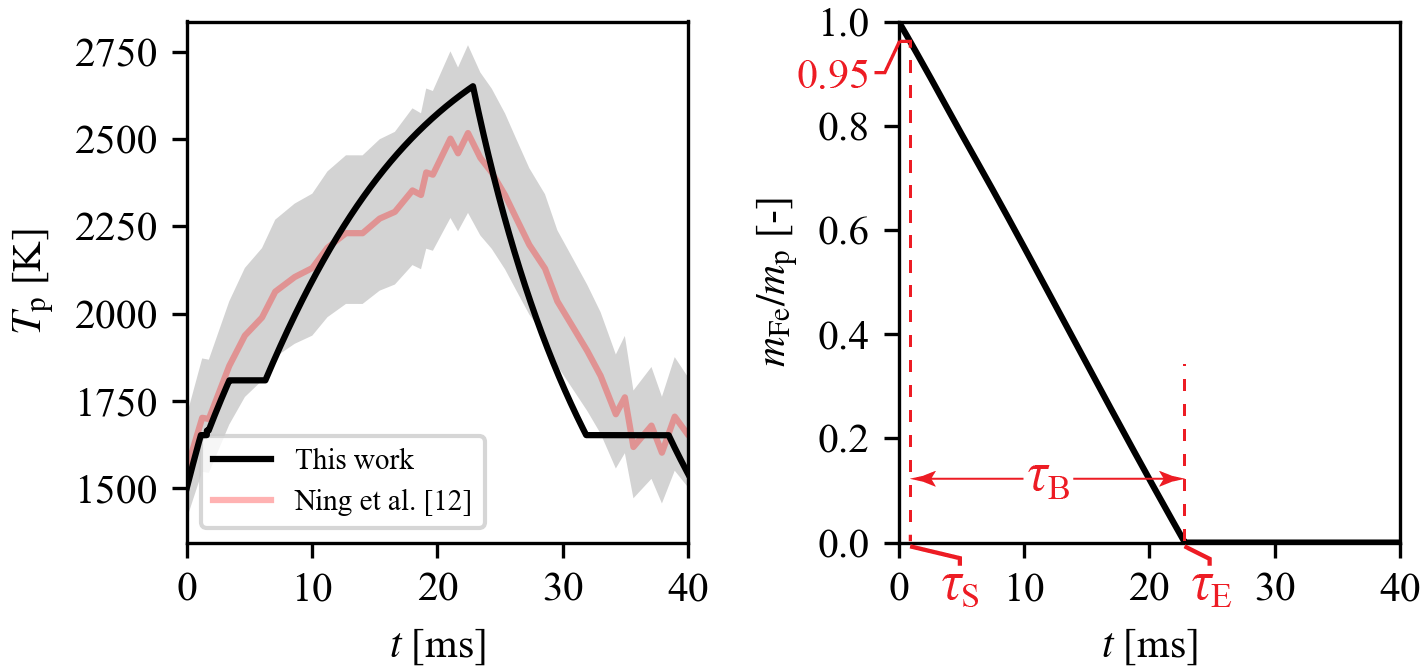
\includegraphics[width=192pt]{final_images/validation.png}
\vspace{1pt}
\caption{\footnotesize \pink Comparison of single particle model vs. experimental data from Ning et al. \cite{Ning}; red line indicates data from Ning et al. and the grey area indicates $\pm$10\% variation from the data}
\label{fig:validation}
\end{figure}
}

\iffalse

\subsection{Particle-gas Coupling}
Trilinear interpolation is used to apply the source terms that are located at particle location to the gas-phase Eulerian grid. Particle drag and heat transfer are coupled to the source terms of the gas-phase energy equation. Coupling of the drag is achieved through forcing an acceleration with the same value as in Eq. \ref{eq:particledrag} but in the vector opposite direction. Coupling of the heat transfer is done through forcing the negative of the change in particle enthalpy, as in Eq. \ref{eq:enthalpy}. The mass of $\mathrm{O_2}$ consumed given in Eq. \ref{eq:mo2} is similarly coupled to the gas-phase species conservation equations.  

\fi 

\section{Simulation Setup}\label{sec:simsetup}\addvspace{10pt}

The present work aims to establish a canonical flow scenario for the combustion of $\mrm{Fe}$ particles that can model flow-particle interaction with adequate control over the flow, particle motion, and reaction parameters. For this purpose, a mixing layer is chosen as the flow scenario as it is well-documented in literature regarding particle-laden reacting multiphase flows such as studies on coal dust combustion \cite{rieth2018carrier}. A mixing layer consists of two streams of gas at different temperatures and velocities-- referred to as ``hot" and ``cold" streams. The iron particles are initially distributed randomly in the cold stream.

In the present work, simulations of a particle-laden mixing layer are used to qualitatively and quantitatively describe the preferential concentration of reacting $\mrm{Fe}$ particles. To initiate research on this topic, the present work focuses on correlating the effect of preferential concentration on the combustion process to the particle size, and hence, all other thermophysical properties are kept constant. \iffalse Preferential concentration is strongly tied to the Stokes number $\mrm{St}$ of the particle-laden flow, and hence, the remaining aspects of the mixing layer such as the flow velocity and the stream temperatures are kept constant. \fi We use a cubical domain of size $L = \SI{22}{mm}$ in the $x$--, $y$-- and $z$--axes. The cold stream is situated in the center of the domain along the $y$--axis with bounds $L_y/4 < y < 3L_y/4$. The hot stream is located in the upper and lower parts of the domain with bounds $y<L_y/4$ and $y>3L_y/4$. Hence, the thickness of the mixing layer is assumed to be $\mathcal{L}= L_y/2 = \SI{11}{mm}$ with dimensions similar to the input nozzle in a typical turbulent iron powder combustor \cite{baigmohammadi2023towards}. Periodic boundary conditions are implemented on all faces of the domain. 

% We consider the following particle sizes $d_\mrm{p} = [14,0,28,39,55]\SI{}{\micro\meter}$ with a domain size of $L=\SI{11}{\milli\meter}$. The selection of these parameters are motivated by typical iron particle sizes in large scale combustors, and typical nozzle sizes. The configuration of the simulations is described in more detail as follows.


\subsection{Gas-phase Thermophysical Properties}\addvspace{10pt}

Air with species mass fractions of $Y_\mathrm{N_2} = 0.76763$ and $Y_\mathrm{O_2} = 0.23237$ is used for both the hot and cold streams. No other gaseous species are incorporated in the simulations. 
The pressure in the domain is set initially at a pressure of $p = \SI{101.325}{\kilo\pascal}$. The velocity of the cold stream is initially set at $u_\mathrm{c} = \SI{2.5}{\meter/\second}$ and the hot stream at $u_\mathrm{h} = \SI{-22.5}{\meter/\second}$, both in the $x$-direction. The velocity of the streams in the normal $y$-- and $z$--directions is set to zero. Hence, a typical velocity scale for the mixing layer is determined from the relative velocity as $\mathcal{U} = |u_\mathrm{h} - u_\mathrm{c}| = \SI{20}{\meter/\second}$.
The temperature of the hot and cold streams are set at $T_\mathrm{c} = \SI{900}{\kelvin}$ and $T_\mathrm{h} = \SI{2000}{\kelvin}$, respectively. {\orange The scenario closely resembles the inlet nozzle of a typical large-scale combustor -- where the hot stream resembles the conditions inside the combustor and the cold stream the feed of $\mathrm{Fe}$ particles into the combustor.
From the chosen thermophysical properties, the bulk Reynolds number is determined to be $\mathrm{Re} = \mathcal{U}\mathcal{L}/\nu_\mrm{f} \approx 2830$ where $\nu_\mrm{f}$ is the mean kinematic viscosity of the two streams. In all the simulations in this study, the gas-phase thermophysical properties are not changed to keep the bulk flow similar. The Reynolds number of the imposed mixing layer is not turbulent, however, the inclusion of particles adds additional momentum via particle drag to the cold stream.} \iffalse The temperature of the cold stream was chosen arbitrarily as $T_\mathrm{c} = \SI{900}{\kelvin}$, whereas the temperature of the hot stream is calculated from the mean enthalpy of the gas to be the temperature that ignites \fi
\begin{figure}[h!]
\centering
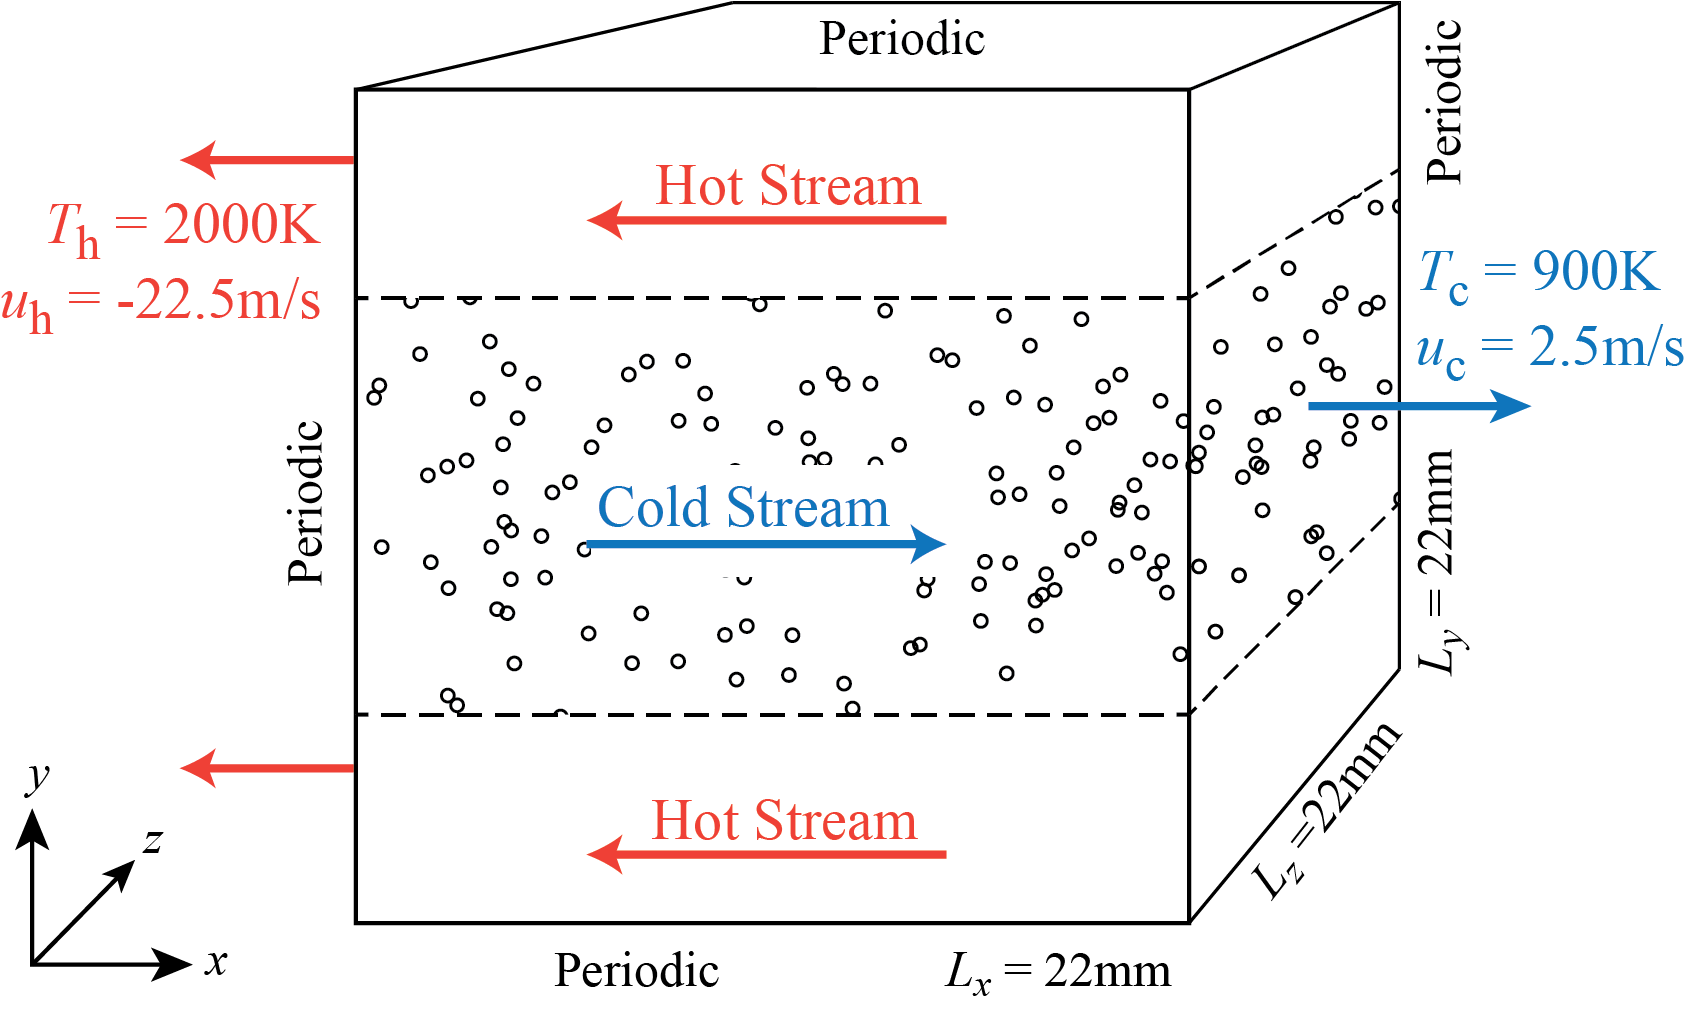
\includegraphics[width=182pt]{images/flowsetup2.png}
\vspace{1pt}
\caption{\footnotesize Domain configuration for the simulations}
\label{fig:flowsetup}
\end{figure}

\subsection{Particle Configuration}\addvspace{10pt}

In this study, the range of particle sizes considered are $d_\mrm{p} = [14,20,28,39,55]\ \SI{}{\micro\meter}$ spanning across sizes that are typically used in a turbulent iron combustor. Monodispersity is assumed for each case. To determine the number of particles for each case, a fuel equivalence ratio of $\phi = 1$ is assumed over the whole domain, and the required mass of Fe is computed using stoichiometry. To isolate the effects of Fe combustion on the flow dynamics, simulations with inert particles are also executed for all particle sizes.\iffalse The total mass of oxygen gas in the domain is computed as:
\begin{equation}\label{eq:mo2}
\begin{split}
    m_\mrm{O_2} &= m_\mrm{O_2,h} + m_\mrm{O_2,c}\\
    &= \left( \rho_\mrm{g,c} + \rho_\mrm{g,h} \right)\cdot Y_\mrm{O_2} \frac{V}{2} 
\end{split}
\end{equation}
where $V$ is the domain volume and the subscripts $\mrm{h}$ and $\mrm{c}$ denote the hot and cold stream properties, respectively. The required mass of $\mrm{Fe}$ with the assumption of stoichiometry is given by:
\begin{equation}
    m_\mrm{Fe} = m_\mrm{O_2} \times \frac{2\cdot W_\mrm{Fe}}{W_\mrm{O_2}} \label{eq:mfe}
\end{equation}

The mass of a single $\mrm{Fe}$ particle is given by:
\begin{equation}
    m_\mrm{p} = \rho_{\mrm{Fe}} \cdot \frac{\pi d_\mrm{p}^3}{6} \label{eq:mp}
\end{equation}
with $\rho_\mrm{Fe} = \SI{7874}{\kilogram/\meter^3}$ as the density of $\mrm{Fe}$. The number of particles can then be calculated using Eq. \ref{eq:mo2}, \ref{eq:mfe} and \ref{eq:mp} as:
\begin{equation}
    n_\mrm{ptcl} = \frac{m_\mrm{Fe}}{m_\mrm{p}} \label{eq:nptcl}
\end{equation}
\fi

Table \ref{tab:dp&lp} presents the particle sizes and number of particles in different simulations performed in this study, along with the mean interparticle distance $\bar{\delta}$ and the single particle burn time $\tau_\mrm{B,0}$. {\red The discreteness parameter, defined in by Lam et al.~\cite{lam2017front,lam2020dimensional} as $\chi = \tau_\mrm{B,0} \alpha_\mrm{f} / \bar{\delta}^2$ where $\alpha_\mrm{f}$ is the thermal conductivity of the gas, is computed to be ranging from $\chi \approx 5$ to $\chi \approx 13.5$ for $\alpha_\mrm{f}$ at $T_\mrm{f}=\SI{2000}{\kelvin}$ to $T_\mrm{f}=\SI{3500}{\kelvin}$, indicating a discrete combustion mode.} The particles are initially distributed randomly in the cold stream, at the cold stream temperature of $T_\mrm{p}= T_\mrm{c} = \SI{900}{K}$ and the cold stream velocity of $u_{\mrm{p}} = u_{\mrm{c}} = \SI{2.5}{\meter/\second}$ in the $x$-direction. {\red The Stokes number at the flow length scale $\mathcal{L}$ for a given particle size can be computed as 

\begin{equation}
    \mrm{St}_\mathcal{L} = \frac{\tau_\mathrm{p}}{\tau_\mathrm{f}}
\end{equation}

\noindent where $\tau_\mathrm{p} = \rho_\mathrm{p} d_\mathrm{p}^2/18\mu_\mathrm{f}$ is the particle relaxation time with $\mu_\mathrm{f}$ the mean dynamic viscosity  and $\tau_\mathrm{f} = {\mathcal{L}}/{\mathcal{U}}$ is the flow timescale. The initial Stokes number $\mrm{St}_{\mathcal{L},0}$ for the particle sizes considered in this study is also presented in Table \ref{tab:dp&lp}.}

\subsection{Grid Resolution}\addvspace{10pt}

 The grid is resolved using 121 nodes in all three directions, resulting in a grid resolution of $\Delta x = \SI{183.33}{\micro\meter}$ and $N=1,728,000$ cells. {\green No turbulence enforcing scheme is employed, rather any dynamic behavior of flow is particle-induced. This choice is made under the assumption that the particle drag would be sufficient in perturbing the mixing layer as is the case in the region close to an inlet nozzle of a typical iron powder combustor. While the flow may be under-resolved in this case, qualitative comparisons can be made with the flow regimes that can be observed for the range of particle sizes considered in this study.}

\iffalse
\subsubsection{Computational configuration}
The computational domain is parallelized in $x$-, $y$- and $z$-directions using $N_\mrm{proc} = [8,8,8]$ processors, respectively. The solver 

The simulations were carried out for a total flow time of $\SI{90}{ms}$. 
\fi

\subsection{Post-processing \& Analysis Setup} \label{sec:postproc}\addvspace{10pt}

In addition to the thermophysical and positional properties of the particle, the start time and the end time of combustion in terms of flow time were also saved as simulation output. The start time of combustion $\tau_\mathrm{S}$ is defined to be the time at which the mass fraction of $\mrm{Fe}$ in the particle crosses below 95\%. The end time of combustion $\tau_\mathrm{E}$ is defined to be the time at which the total mass of $\mrm{Fe}$ is completely oxidized. The burn time $\tau_\mathrm{B}$ is then computed for each particle as the difference between the end and the start times. A visual representation of $\tau_\mathrm{S}$, $\tau_\mathrm{E}$ and $\tau_\mathrm{B}$ can be seen in Figure \ref{fig:validation}.

\begin{figure}[h!]
\centering
\vspace{-12pt}
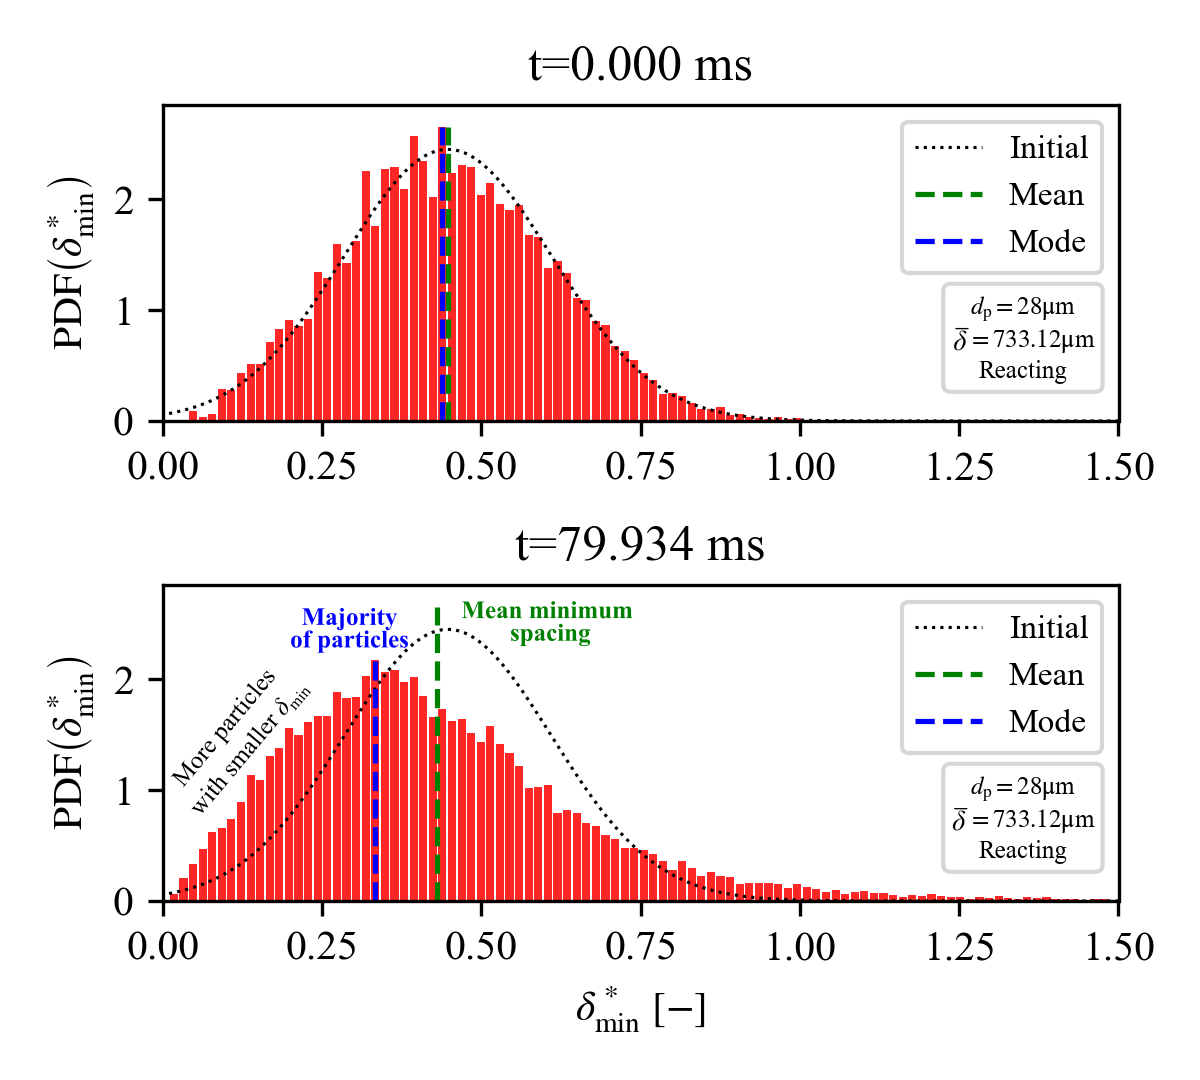
\includegraphics[width=195pt]{final_images/pdfhistogram_annotated.png}
\caption{\footnotesize \pink PDF of normalized minimum spacing of particles $\delta_\mrm{min}^*$ at two different flow times. The mean and mode of the distribution are computed and saved at every timestep.}
\label{fig:pdfhistogram}
\end{figure}

For each particle size, the mean interparticle distance $\bar{\delta}$ can be computed from the particle number density as:
\begin{equation}
    \bar{\delta} = \left( \frac{n_\mrm{ptcl}}{V}\right)^{-1/3} \label{eq:lp}
\end{equation}

In this study, the minimum spacing $\delta_\mrm{min}$ is used in the statistical analysis of particle clustering. $\delta_\mrm{min}$ of each particle is the distance to its nearest neighbor. For each particle, $\delta_\mrm{min}$ is computed at each saved output step using a KD-tree analysis of the particle locations in the Cartesian domain. To compare $\delta_\mrm{min}$ across different cases, $\delta_\mrm{min}$ is normalized by the mean interparticle distance $\bar{\delta}$ to obtain the normalized minimum spacing $\delta_\mrm{min}^*$. 

\begin{equation}
    \delta_\mrm{min}^* = \frac{\delta_\mrm{min}}{\bar{\delta}}
\end{equation}

At each timestep, a histogram of $\delta_\mrm{min}^*$ is generated for the particle distribution, and the mean and the mode of the distribution are computed as represented in Figure \ref{fig:pdfhistogram}. The mean minimum spacing indicates a representative value for the total particle distribution, however, the mode of the distribution may indicate $\delta_\mrm{min}^*$ that is exhibited by a majority of the particles. 



\begin{table}[h!] \footnotesize
\caption{Particle sizes $d_\mrm{p}$, the corresponding mean interparticle distance $\bar{\delta}$, the number of particles $n_\mrm{ptcl}$ simulated}, the initial Stokes number $\mrm{St}_{\mathcal{L},0}$ of each particle size and the corresponding single-particle burn time $\tau_{\mrm{B,0}}$

\renewcommand{\arraystretch}{1}
\vspace{6pt}

\centerline{\begin{tabular}{c>{\hspace{-3pt}}c>{\hspace{-3pt}}c>{\hspace{-3pt}}c>{\hspace{-3pt}}c}
\hline
\rule{0pt}{1em}$d_\mrm{p}$ [$\SI{}{\micro\meter}$]                       & $\bar{\delta}$ [$\SI{}{\micro\meter}$]  & $n_\mrm{ptcl}$ [-]  & \red{$\mrm{St}_{\mathcal{L},0}$} [-] & $\tau_\mathrm{B,0}$ [ms]  \\
\hline
14                                  & 366.56   & 216000 & {\red 1.87}   &  1.32 \\
20                               & 523.66   &  74000  & {\red 3.82}  & 2.69 \\
28                              & 733.12   & 26800  & {\red 7.49} & 5.28\\ 
39                              & 1021.13   &  10000  & {\red 14.52} & 10.26\\ 
55                               & 1440.05   & 3600  & {\red 28.89} & 20.39\\
\hline 
\end{tabular}}
\label{tab:dp&lp}
\end{table}



For a statistically uniform distribution of particles, the probability density function (PDF) of the normalized minimum spacing $\delta_\mrm{min}^*$ will have a mean value at $0.5539$ \cite{haenggi2005distances}. However, as the particles are initialized in a volume one-half of the domain (cold stream), the initial mean value for the PDF of $\delta_\mrm{min}^*$ following Eq. \ref{eq:lp} would be $ 0.5539 \times \left( 2 \right)^{-1/3}\approx 0.4396$.


To observe the effect of clustering on the burn time of the particle, the minimum spacing for each particle is also averaged temporally over the flow time to obtain the temporal mean of the minimum spacing $\langle \delta_\mrm{min}^* \rangle$. 


\section{Results \& Discussion}\addvspace{10pt}

\subsection{Combustion Regime}\addvspace{10pt}

\iffalse 
\begin{figure*}[h!]
\centering
\vspace{-0.4 in}
\includegraphics[width=\textwidth]{images/temp2d.png}
\vspace{10 pt}
\caption{\footnotesize Engine configuration (top view).}
\label{fig:temp}
\end{figure*}

\begin{figure*}[h!]
\centering
\vspace{-0.4 in}
\includegraphics[width=\textwidth]{images/yo2_2d.png}
\vspace{10 pt}
\caption{\footnotesize Engine configuration (top view).}
\label{fig:yo2}
\end{figure*}
\fi

\iffalse
\begin{figure}[h!]
\centering
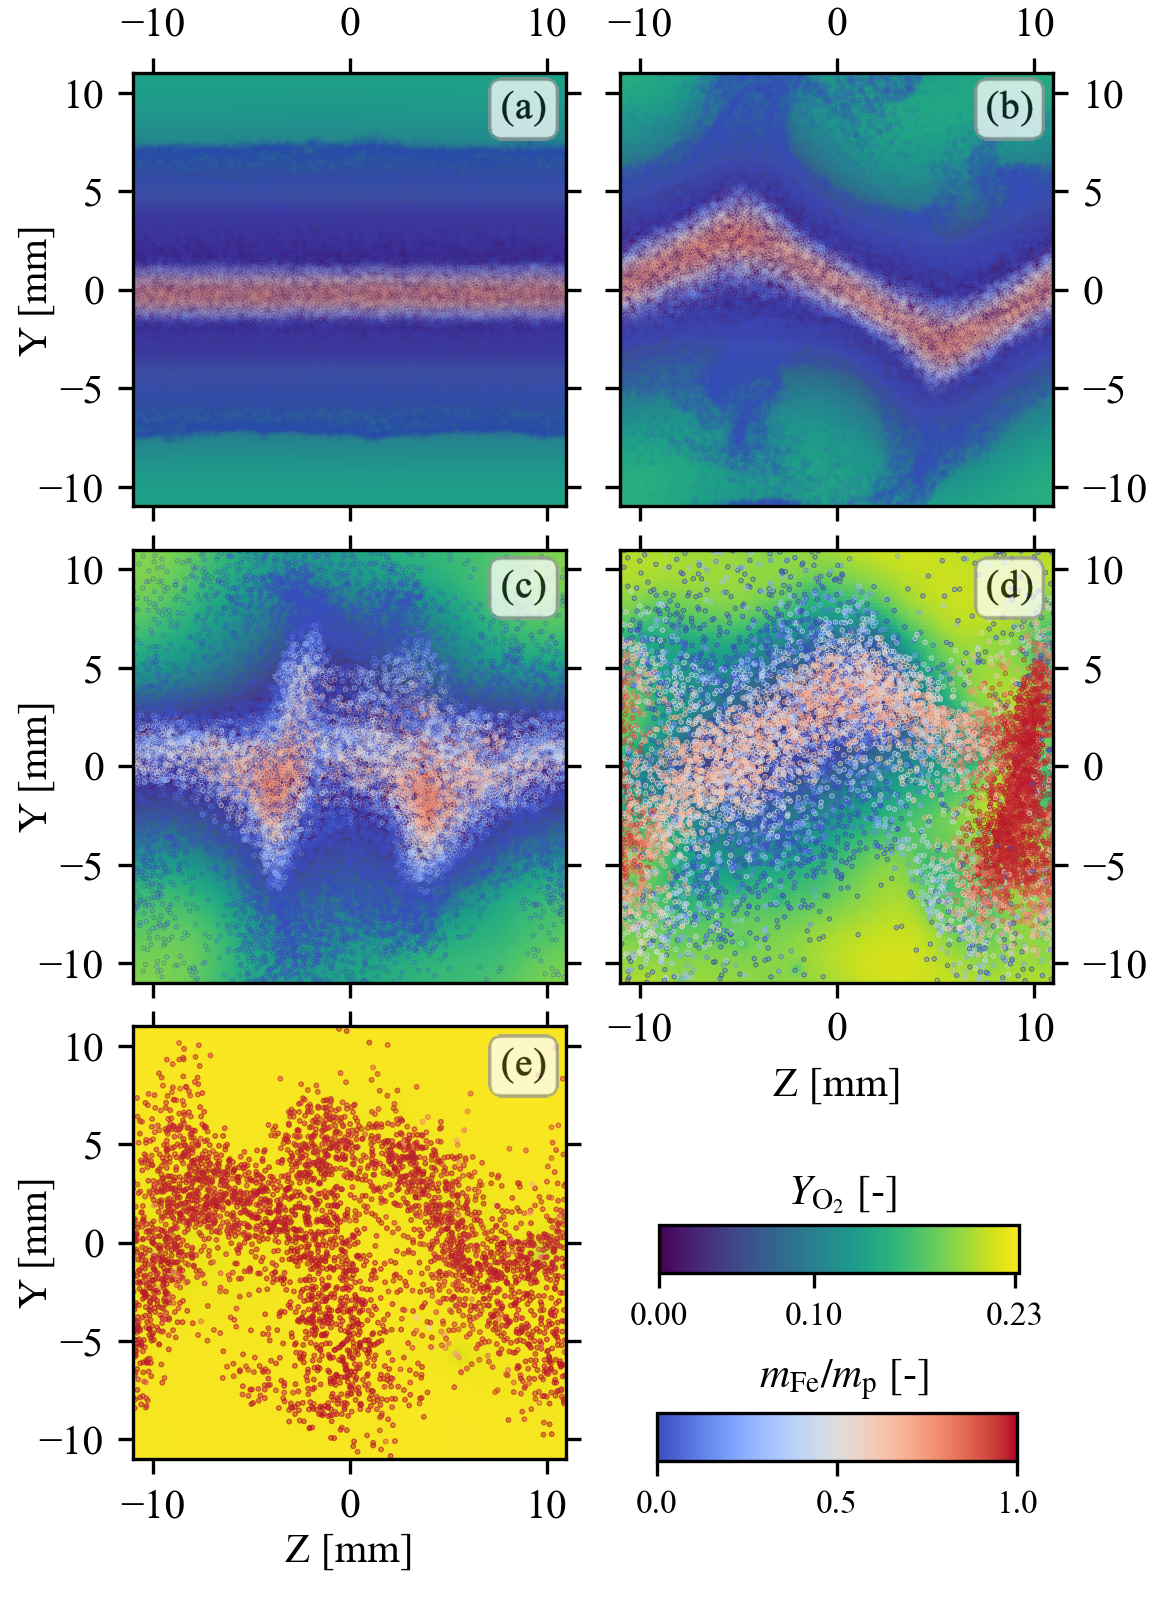
\includegraphics[width=192pt]{images/yo2_plots_2.png}
\caption{\footnotesize Gas-phase field of mass fraction $Y_{\mrm{O_2}}$ and particle $\mrm{Fe}$ mass fraction $m_\mrm{Fe}/m_\mrm{p}$ at a flow time of $t=\SI{40}{\milli\second}$. Subfigures [a,b,c,d,e] correspond to particle diameters $d_\mrm{p} = [14,20,28,39,55]\ \SI{}{\micro\meter}$, respectively.}
\label{fig:yo2}
\end{figure}
\fi

Figure \ref{fig:temp} shows the gas phase and particle temperatures at a flow time of $t=\SI{40}{\milli\second}$. The gas-phase fields are visualized in a central plane normal to the flow direction ($yz$-plane with the mean flow in the $x$-direction). From Figure \ref{fig:temp}, a clear difference can be seen in cases with smaller particle sizes $d_\mrm{p}\leq\SI{20}{\micro\meter}$ and the larger particle sizes $d_\mrm{p}\geq\SI{28}{\micro\meter}$. A flame front is seen with the smallest particle size considered in this study, and there is no perturbation of the mixing layer. However, larger particles destabilize the mixing layer easily and this gives rise to a strong flow-particle interaction, resulting in dynamic particle motion and complex effects. {\pink With $d_\mrm{p} \geq \SI{28}{\micro\meter}$, the initial structure of the mixing layer is altered completely. Hence, two flow regimes are observed -- a \textit{laminar-like} behavior for smaller particles, and a \textit{turbulent-like} behavior for the larger particles. Additional visualization is made available through supplementary material attached to the manuscript. }


\begin{figure}[h!]
\centering
\includegraphics[width=176pt]{final_images/temp2d.png}
\caption{\footnotesize Gas-phase temperature $T_\mathrm{g}$ fields at a $yz$-midplane in the $x$-direction and particle positions and temperatures $T_\mrm{p}$ at a flow time of $t=\SI{40}{\milli\second}$.}
\label{fig:temp}
\end{figure}

\iffalse
Figure \ref{fig:yo2} shows a localized depletion of $\mrm{O_2}$ in regions of higher concentration of particles. With the cases of $d_\mrm{p} \leq \SI{20}{\micro\meter}$, $Y_\mrm{O_2}$ at the center of the domain is significantly lower compared to the outer parts of the domain. This depletion of $\mrm{O_2}$ is expected to slow down the combustion reaction. Figures \ref{fig:temp} \& \ref{fig:yo2} also show the variation in the timescale of combustion across different particle sizes, with the smallest particles well through the combustion process and the largest particles not yet ignited at $t=\SI{40}{\milli\second}$.


The presence of empty vortices and regions of higher particle concentration can also be seen from the figures \ref{fig:temp}, and a coarse qualitative comparison can be made. Quantification of the clustering of particles is discussed in more detail in Section 4.3\ref{sec:clustering}. \fi

\subsection{Start and End Times of Combustion}
\label{sec:combustionmodes}\addvspace{10pt}

An analysis of the start and end times of combustion of all the particles in regard to the initial $y$-coordinate $|y_0|$ of the particle in the domain is shown in Figure \ref{fig:startend}. Particles of size $d_\mrm{p} =[14,20] \SI{}{\micro\meter}$ show good correlation with $|y_0|$. This can be attributed to the laminar-like behavior keeping the structure of the mixing layer intact. This correlation is substantially weaker for particles of size $d_\mrm{p} = [28,39,55]\SI{}{\micro\meter}$ since the larger particles disperse out of the initial mixing layer structure. 

\begin{figure}[h!]
\centering
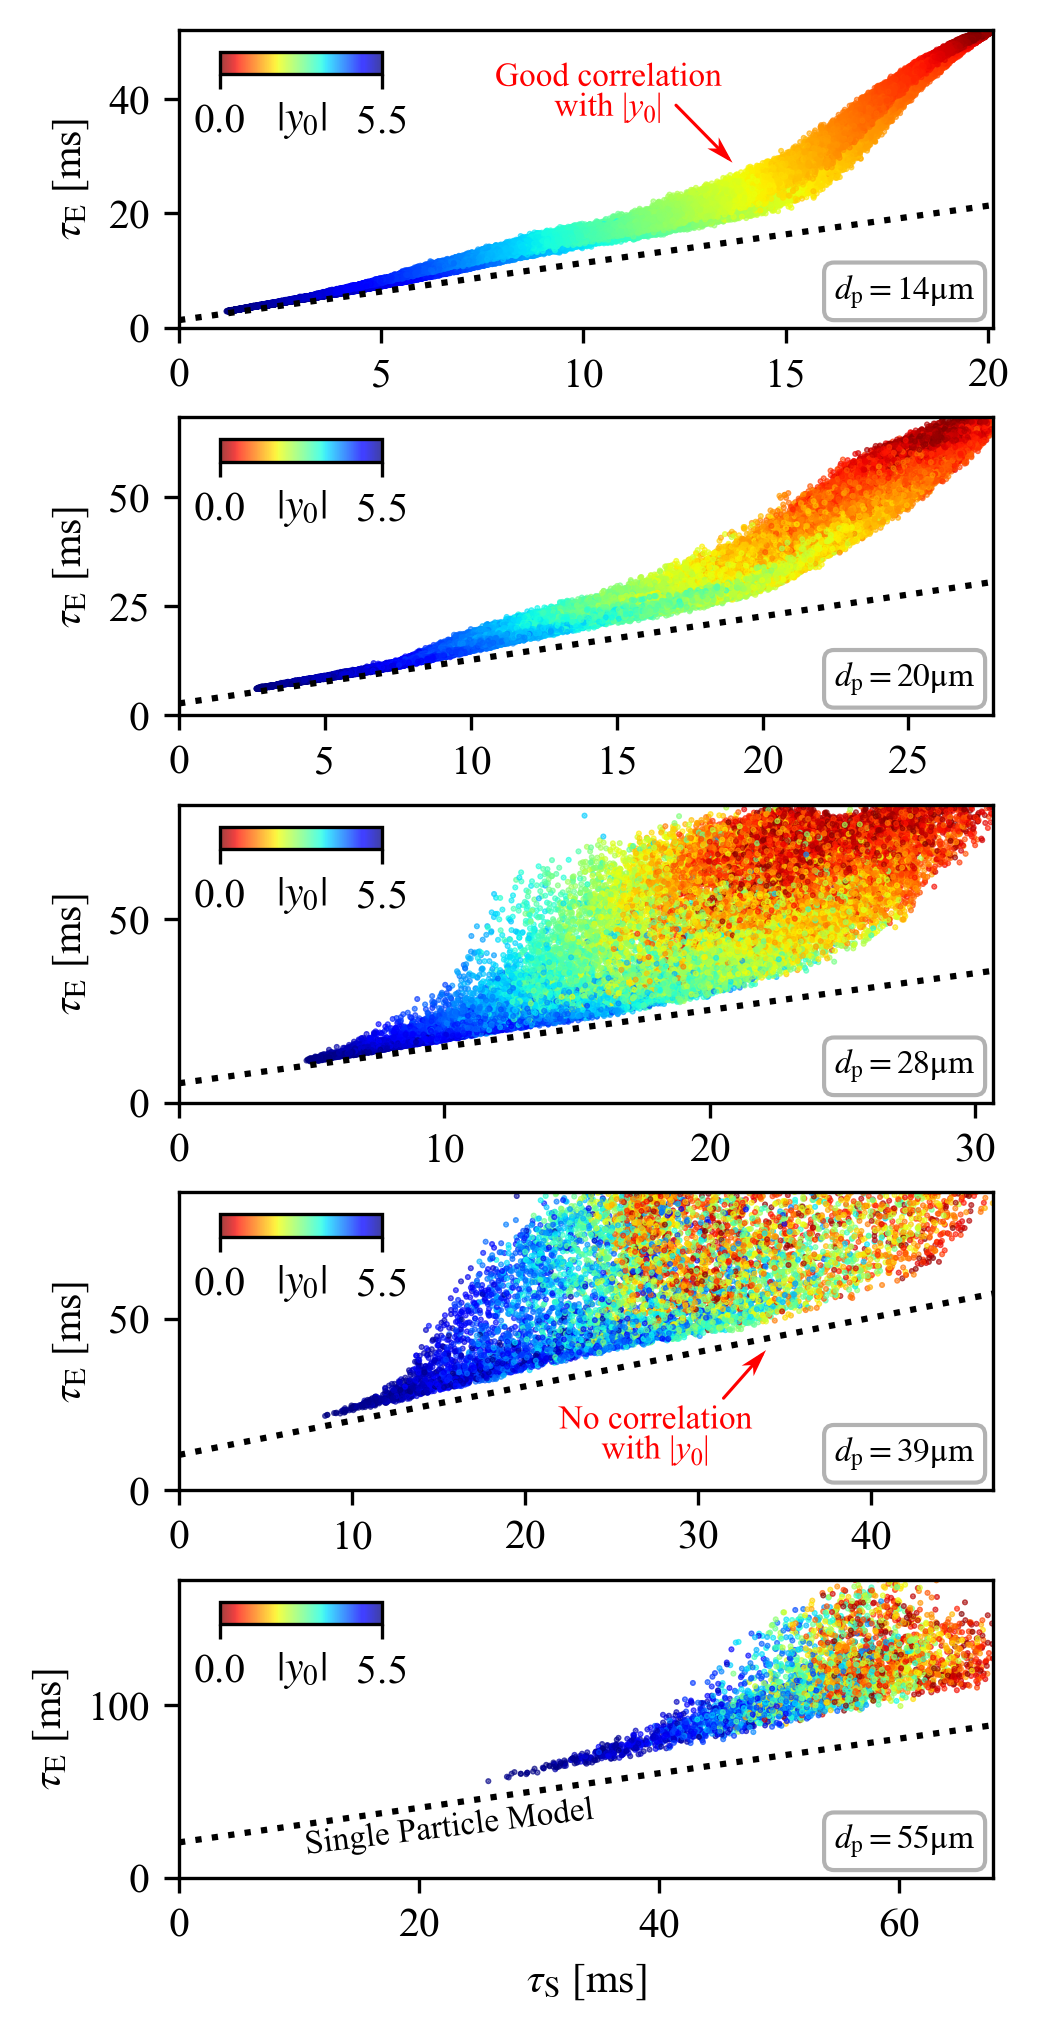
\includegraphics[width=176pt]{final_images/startend_annotated.png}
\caption{\footnotesize Particle combustion start time $\tau_\mathrm{S}$ vs. combustion end time $\tau_{\mrm{E}}$, initial $y$-coordinate of particle $y_0$ in color--zero denotes the center of the domain and 5.5 denotes the interface of the mixing layer. Burn time predicted by a zero-dimensional, single-particle combustion model is represented as a line.}
\label{fig:startend}
\end{figure}



All particle sizes show considerable deviation in the particle end times $\tau_\mrm{E}$ as compared to the combustion end time predicted by the 0D single particle model. The mechanism of the extension in burn time $\tau_\mrm{B}$ is different for the two modes of combustion. This is further discussed in Sections 4.3 and 4.4.

{\pink

\subsection{Analysis of Laminar-like Combustion Mode}\addvspace{10pt}

Visualization of the particle distribution and flow evolution for the simulations with smaller particle sizes portray a laminar-like behavior where a smooth flame can be observed. For particles of size $d_\mrm{p}=\SI{14}{\micro\meter}$, the mixing layer is not perturbed and stays completely laminar as seen in Figure \ref{fig:flame1}. $\SI{20}{\micro\meter}$-sized particles perturb the mixing layer and produce a few plumes at the shear interface as in Figure \ref{fig:flame2}. However, since the single particle burn time $\tau_\mathrm{B,0}$ of $\SI{20}{\micro\meter}$ particles is smaller than the timescale of flow evolution, the plume consists entirely of burnt particles, and the combustion behavior is still laminar-flame-like. In both of these cases, the extension in the burn time of combustion $\tau_\mrm{E}$ as seen in Figure \ref{fig:startend} can be explained through the depletion of $\mrm{O_2}$ in the center of the domain as in Figures \ref{fig:flame1} and \ref{fig:flame2}, and completion of combustion is limited by the mass transport of $\mrm{O_2}$ from the hot stream into the cold stream.

\begin{figure}[h!]
\centering
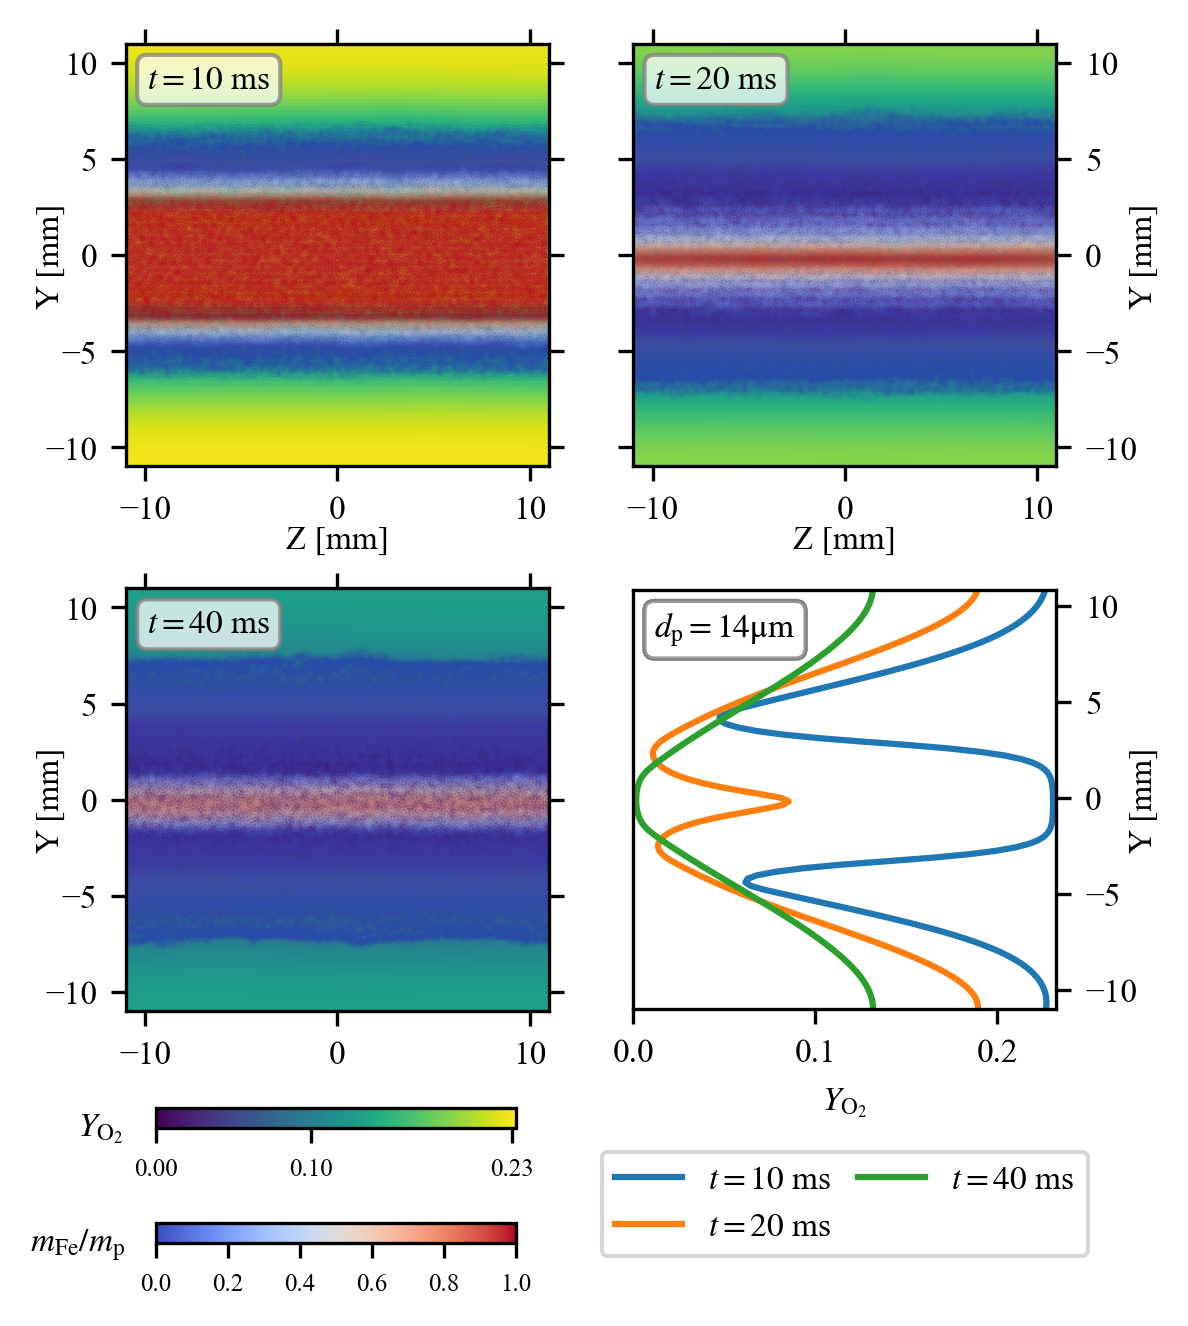
\includegraphics[width=186pt]{final_images/flamepropagation_alt1.png}
\caption{\footnotesize \pink Gas-phase field of mass fraction $Y_{\mrm{O_2}}$ and particle $\mrm{Fe}$ mass fraction $m_\mrm{Fe}/m_\mrm{p}$ of the simulation of $d_\mathrm{p}=\SI{14}{\micro\meter}$ at a flow time of $t=[10,20,40]\mathrm{ms}$. Bottom right figure indicates $xz-$plane-averaged $Y_\mathrm{O_2}$ at $t=[10,20,40]\mathrm{ms}$.}
\label{fig:flame1}
\end{figure}

\begin{figure}[h!]
\centering
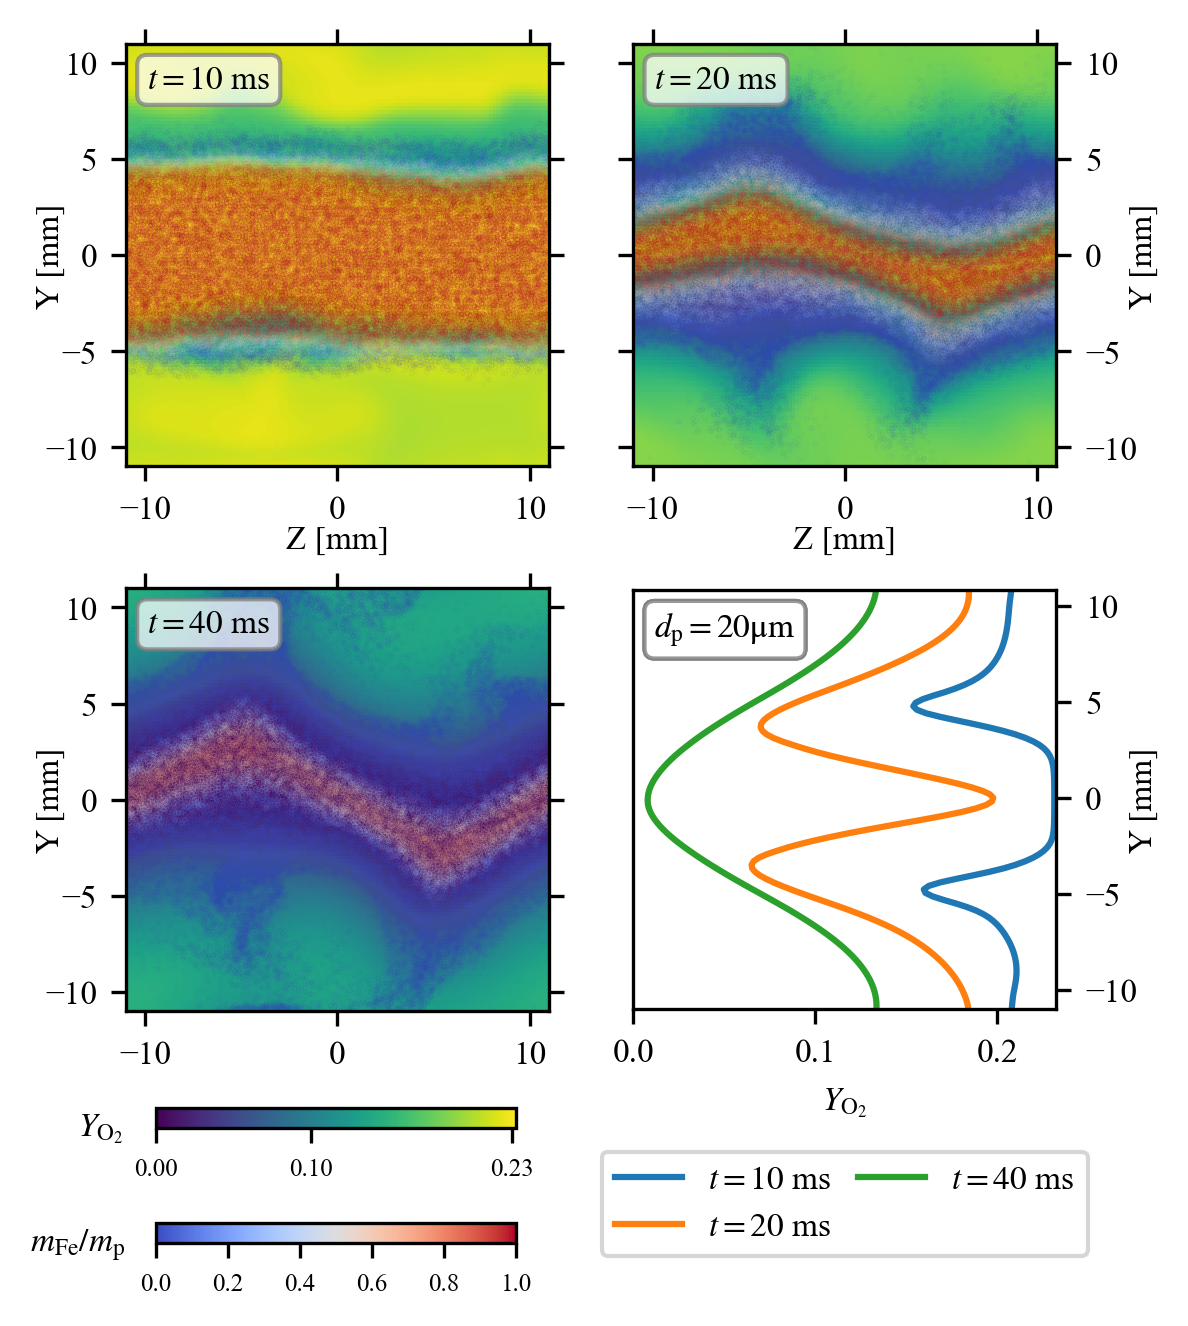
\includegraphics[width=186pt]{final_images/flamepropagation_alt2.png}
\caption{\footnotesize \pink Gas-phase field of mass fraction $Y_{\mrm{O_2}}$ and particle $\mrm{Fe}$ mass fraction $m_\mrm{Fe}/m_\mrm{p}$ of the simulation of $d_\mathrm{p}=\SI{20}{\micro\meter}$ at a flow time of $t=[10,20,40]\mathrm{ms}$. Bottom right figure indicates $xz-$plane-averaged $Y_\mathrm{O_2}$ at $t=[10,20,40]\mathrm{ms}$.}
\label{fig:flame2}
\end{figure}

\subsection{Analysis of Turbulent-like Combustion Mode}\addvspace{10pt}

As evidenced in Figure~\ref{fig:temp} for particles of sizes $d_\mrm{p} \ge \SI{28}{\micro\meter}$, the particle drag is strong enough to perturb the mixing layer which results in turbulence onset. Additionally, the single particle burn time $\tau_\mrm{B,0}$ is sufficiently larger than the timescale of dispersion of particles out of the initial mixing layer structure. Hence, the combustion mode is not laminar-flame-like, but rather discrete. Significant variation in end times for a given start time of combustion is observed for the larger particles in Figure \ref{fig:startend}. Figure \ref{fig:burnymin} shows the correlation of burning time to particle clustering, evaluated as the normalized minimum spacing averaged over the flow time  $\langle \delta_\mrm{min}^* \rangle$. }

\iffalse

The distribution of particles in such a plot portrays the presence of two distinct mechanisms through which the burn time of the particles $\tau_\mathrm{B}$ can be extended -- depletion of oxygen as a consequence of the initial structure of the mixing layer and depletion of oxygen in particle clusters. The two mechanisms can be distinguished through the temporal mean of the minimum spacing $\delta_\mrm{min}^*$ since the first mechanism is purely a consequence of the structure of the mixing layer and does not result in particle clustering. The two mechanisms also differ by their characteristic timescales -- the first mechanism a result of the discrepancy of the single particle burn time and the thermal and mass diffusion timescale, and the second carrying the discrepancy of the clustering timescale and the mass diffusion timescale. Categorization of the various timescales in such flows is essential in furthering this line of analysis and understanding the threshold of preferential concentration better.

\fi

\begin{figure}[h!]
\centering
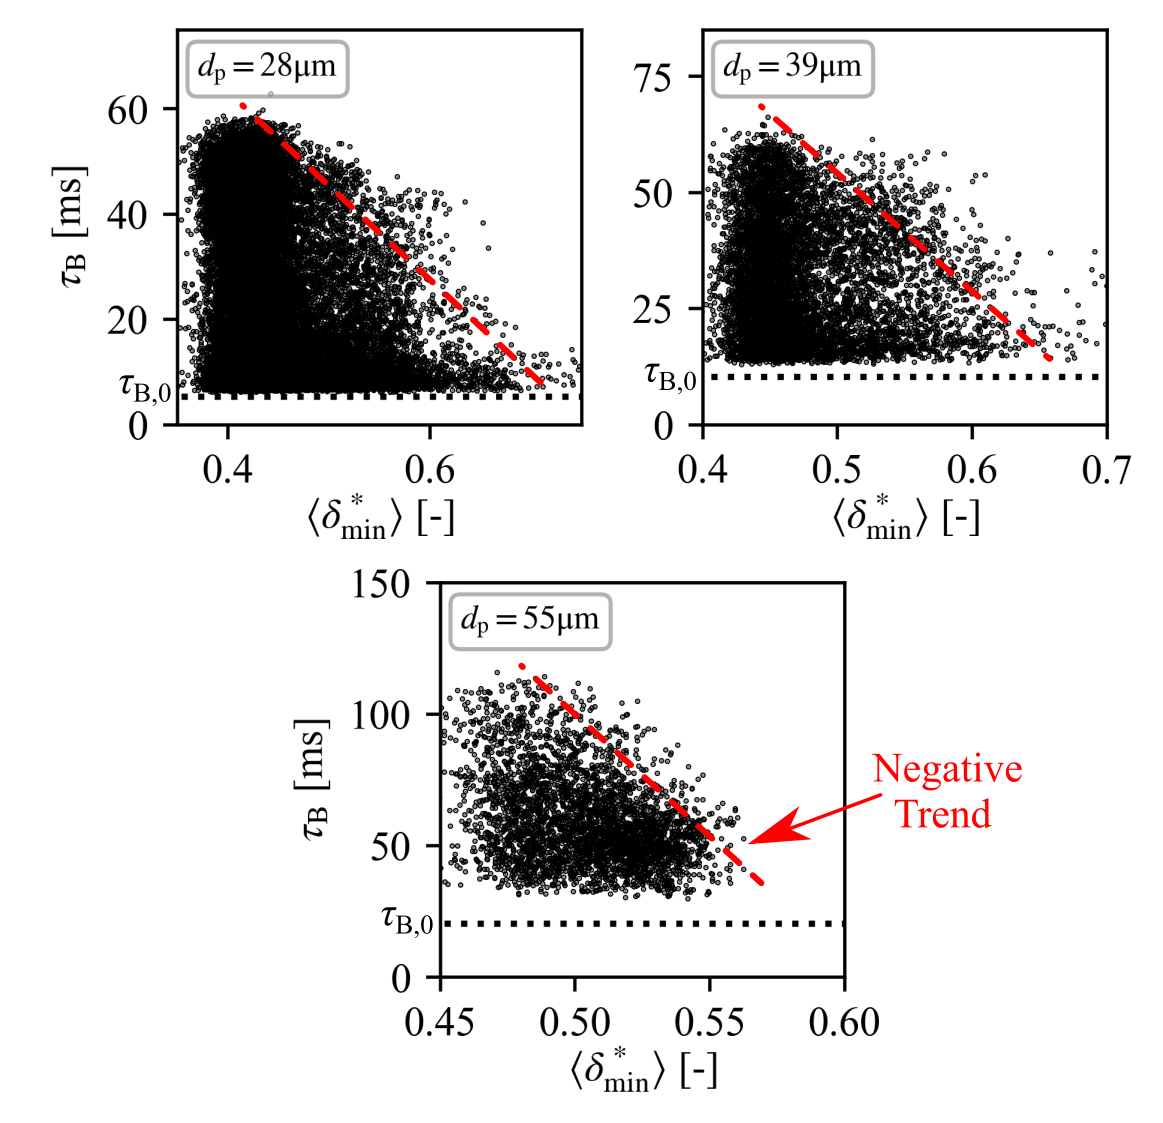
\includegraphics[width=192pt]{final_images/burnymin_annotated4.png}
\caption{\footnotesize Comparing the particle burn times $\tau_\mrm{B}$ with the normalized minimum spacing averaged over the flow time $\langle \delta_\mrm{min}^* \rangle$.}
\label{fig:burnymin}
\end{figure}

\iffalse

For $d_\mrm{p} = \SI{14}{\micro\meter}$, the correlation of the burn times with the start times is observed. However, there is no significant correlation of $\tau_\mrm{B}$ with $\bar{\delta}_\mrm{min}^*$. 

\fi 

The distribution of $\tau_\mrm{B}$ vs. $\langle \delta_\mrm{min}^* \rangle$ is characterized by a negative-sloped trend. Hence, it is inferred that particles that have longer burn times $\tau_\mrm{B}$ are significantly correlated with lower values of the normalized minimum spacing averaged over the flow time $\langle \delta_\mrm{min}^* \rangle$. 

It should be noted that concentrated regions of particles may contain unburnt, burning, or fully burnt particles. However, the correlation of $\tau_\mrm{B}$ vs. $\langle \delta_\mrm{min}^* \rangle$ is indicative of longer burning times owing to a denser particle distribution.

\iffalse

\begin{figure}[h!]
\centering
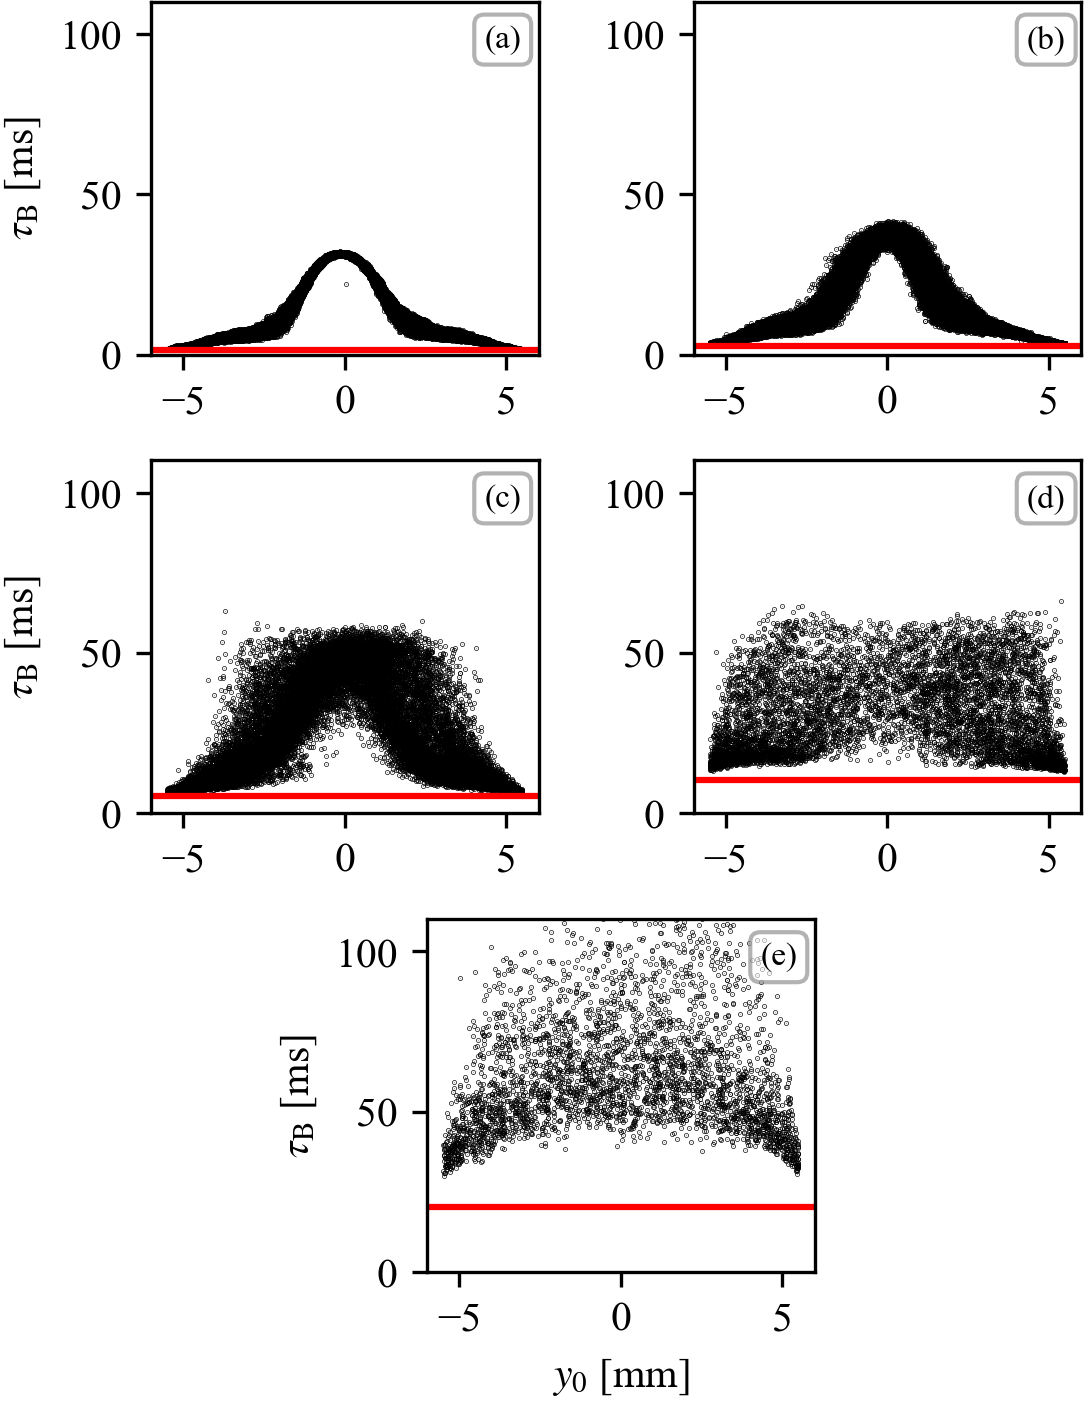
\includegraphics[width=192pt]{images/burnyloc3.png}
\caption{\footnotesize Particle burn time $\tau_\mathrm{B}$ vs. initial $y$-coordinate of particle $y_0$. Subfigures [a,b,c,d,e] correspond to particle diameters $d_\mrm{p} = [14,20,28,39,55]\ \SI{}{\micro\meter}$, respectively.}
\label{fig:burnyloc}
\end{figure} 

\fi

\subsection{Effects of Combustion on Particle Clustering}\label{sec:clustering}\addvspace{10pt}

\iffalse

A qualitative description of the flow-particle interaction effects and the clustering of particles has been established through visualizations of particle positions. The effects of particle clustering on the combustion characteristics of the particles have also been statistically analyzed. 

\fi

Figure \ref{fig:pdfcompare1}  show the temporal evolution of the mean and mode of the normalized minimum spacing $\delta_\mrm{min}^*$ compared to simulations of inert particles of the same sizes. 

Particles exhibiting laminar-like flame behavior do not disperse out of the initial mixing layer structure. Hence, the mean minimum spacing does not tend towards 0.5539. {\blue Particles of size $d_\mrm{p}=\SI{14}{\micro\meter}$ show deviation in the mode of minimum spacing $\delta_\mrm{min}^*$ compared with inert particles as in Figure \ref{fig:pdfcompare1}}. This is a consequence of the thermal expansion of gases at the location of the ``flame front" moving the particles further towards the center of the domain. 

{\blue Mean minimum spacing of particles exhibiting turbulent-like behavior steadily increases towards 0.5539 as seen in Figure \ref{fig:pdfcompare1}, however, in the case of reacting $\SI{39}{\micro\meter}$ particles, the mean minimum spacing decreases after sufficient particles have completely burnt out. This deviation can be attributed to the modification of particle relaxation time $\tau_\mrm{p}$ and the flow timescale $\tau_\mrm{f}$ as a result of combustion (i.e., an increase in viscosity at higher gas temperatures).}

{\orange The burnt particles possess a larger size $d_\mrm{p,end}$ that can be determined through stoichiometry as $d_\mrm{p,end} / d_\mrm{p} \approx 1.2081$. However, the mass density of FeO is smaller than that of Fe i.e., $\rho_\mrm{FeO} / \rho_\mrm{Fe} \approx 0.73$. Combustion of particles heats up the gas, which increases the gas viscosity $\mu_\mrm{f}$. On comparing the dynamic viscosity of air at $\SI{900}{\kelvin}$ and $\SI{2500}{K}$, it was found that $\mu_\mrm{f,900K} / \mu_\mrm{f,2500K} \approx 2.023$. These effects result in a decrease in the particle relaxation time $\tau_\mrm{p,end} / \tau_\mrm{p} \approx 0.526$ as the particle burns. The flow that is simulated portrays decaying turbulence without any relevant carrier-phase enforcing, and hence, the flow timescale $\tau_\mrm{f}$ is expected to increase over time. Additionally, an increase in gas viscosity reduces the flow Reynolds number, which results in a further increase in $\tau_\mrm{f}$. Hence, it is hypothesized that the combustion of particles results in a decrease in the Stokes number.}

\iffalse 

It can then be observed from Figure \ref{fig:pdfcompare} that particles of sizes $d_\mrm{p} = \SI{20}{\micro\meter}$ homogenize faster after completion of combustion, whereas particles of sizes $d_\mrm{p} = \SI{28}{\micro\meter}$ homogenize slower. The longer burn time of larger particles $d_\mathrm{p} = \SI{55}{\micro\meter}$ results in similar statistics as that of inert particles up to a flow time of $t=\SI{80}{\milli\second}$ considered in this analysis. 

From this, it can be inferred that for the chosen set of thermophysical properties, particles of sizes in the range $\SI{20}{\micro\meter} < d_\mrm{p} < \SI{28}{\micro\meter}$ possess an effective Stokes number $\mrm{St}_\mrm{eff} \approx 1$. Further analysis on quantifying and comparing flow, particle, and reaction timescales would be beneficial in a complete understanding of the particle-flow dynamics.


This might be an indication that the particle, flow, and reaction timescales are in the same order of magnitude that resulting in enhancement of the preferential concentration effect, i.e., $\mathrm{St}\approx 1$. \fi  

\iffalse
It is also noted that, for particle sizes $d_\mrm{p} \geq \SI{39}{\micro\meter}$, the decrease in $\delta_\mrm{min}^*$ does not correspond to the timescale of particle combustion. Hence, it can be hypothesized that the clustering of larger particles is accelerated more by the perturbation and instability of the mixing layer and less by the effect of particle combustion on the flow. Further research is required to isolate the effect of particle combustion on the flow, and subsequently on particle motion and distribution. \fi   

\begin{figure}[h!]
\centering
\hspace{-7pt}
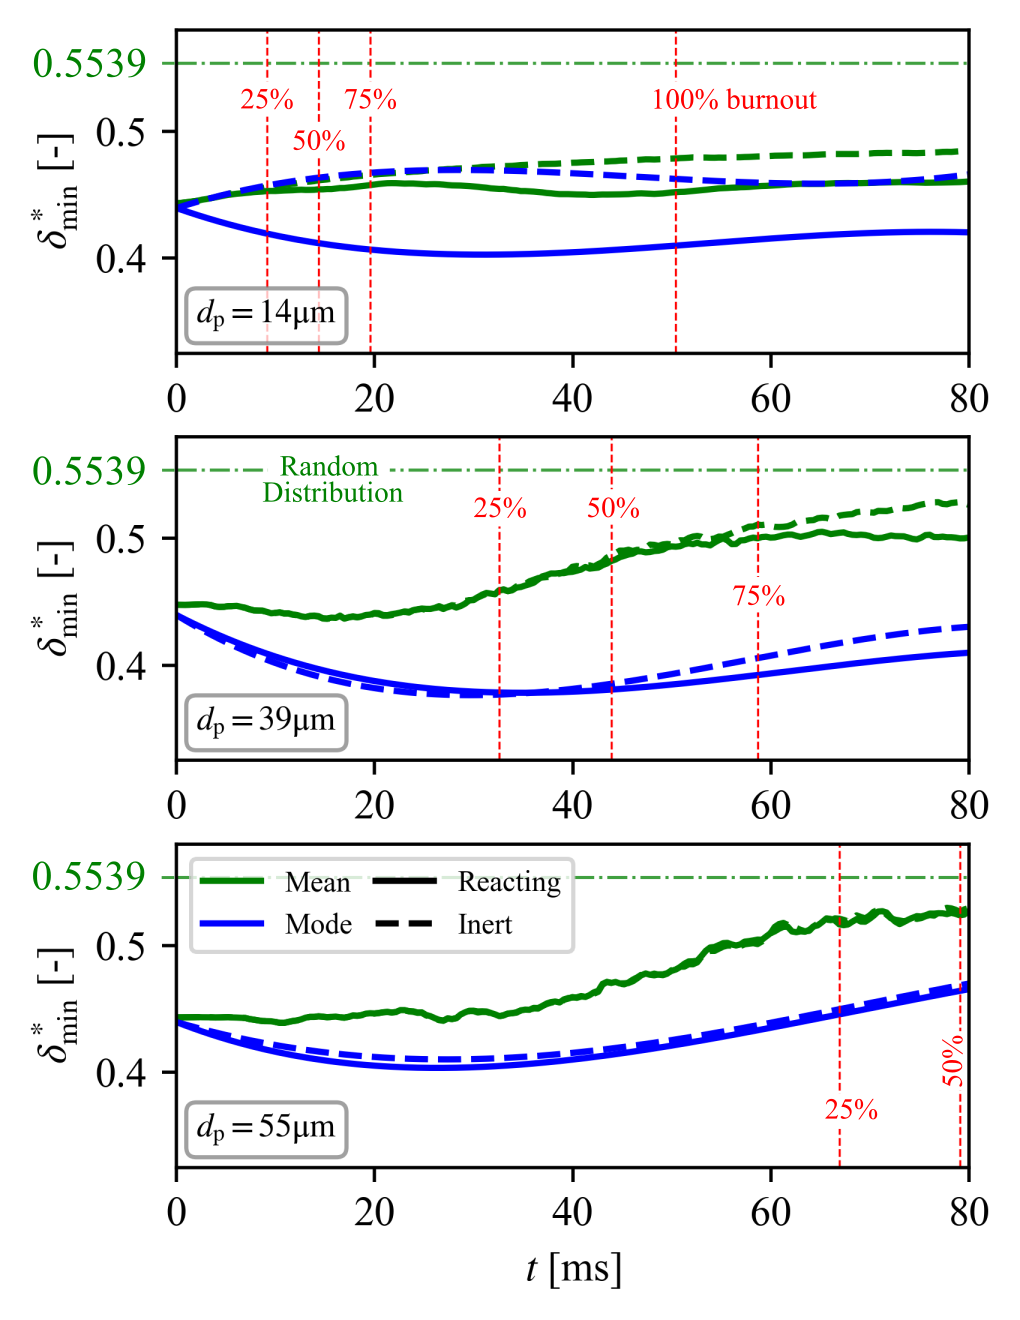
\includegraphics[width=176pt]{final_images/meanminimumspacing3a.png}
\caption{\footnotesize \pink Mean and mode of the minimum spacing of particle distribution $\delta_\mrm{min}^*$ vs. flow time $t$, compared between reacting and inert particles, for particle size $d_\mrm{p} = [14,39,55]\SI{}{\micro\meter}$. Annotations in red indicate the Fe burnout time. The green dashed line at $\delta_\mrm{min}^* = 0.5539$ indicates the mean value if particles were dispersed all over the domain randomly.}
\label{fig:pdfcompare1}
\end{figure}

% \begin{figure}[h!]
% \centering
% \hspace{-7pt}
% 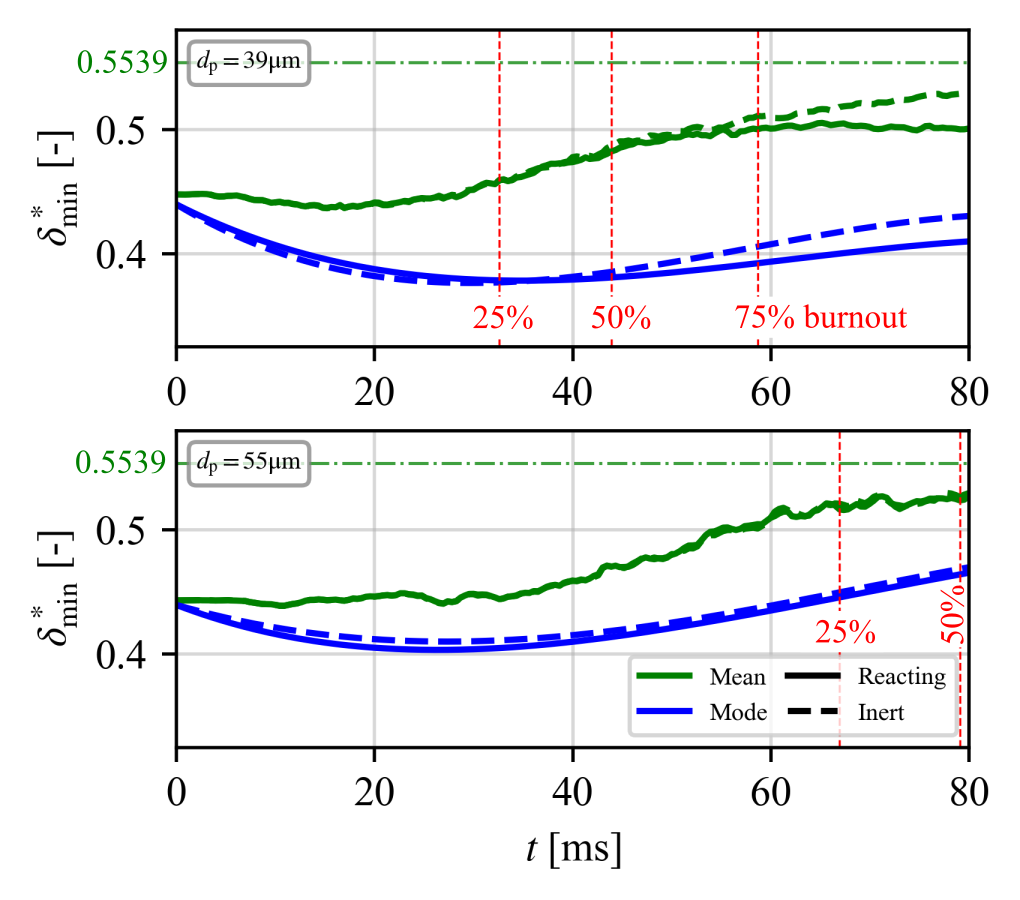
\includegraphics[width=176pt]{final_images/meanminimumspacing2a.png}
% \caption{\footnotesize \pink Mean and mode of the minimum spacing of particle distribution $\delta_\mrm{min}^*$ vs. flow time $t$, compared between reacting and inert particles, for particle sizes $d_\mrm{p} = \SI{39}{\micro\meter}$ （top) and $d_\mrm{p} = \SI{55}{\micro\meter}$ (bottom). Annotations in red indicate the Fe burnout time. The green dashed line at $\delta_\mrm{min}^* = 0.5539$ indicates the mean value if particles were dispersed all over the domain randomly.}
% \label{fig:pdfcompare2}
% \end{figure}

\section{Conclusion}
\label{sec:conclusion}
\addvspace{10pt}

In the present work, the interplay between preferential concentration in turbulence induced by shear flows and the combustion characteristics of iron particles of different sizes $d_\mrm{p} = [14,20,28,39,55]\ \SI{}{\micro\meter}$ is studied. Smaller particles $d_\mrm{p} \leq \SI{20}{\micro\meter}$ burn in a laminar-like flow regime, retain the structure of the mixing layer, and have particle burn times $\tau_\mrm{B}$ that are statistically correlated with the initial location of the particle in the mixing layer. Larger particles $d_\mrm{p} \geq \SI{28}{\micro\meter}$ disperse out of the mixing layer and burn in a turbulent-like flow regime. Further analysis of the normalized minimum spacing $\delta_\mrm{min}^*$ for each particle indicates that the particles with longer burn times have lower values of minimum spacing averaged over the flow time $\langle \delta_\mrm{min}^* \rangle$. 

A comparison of the mean and mode of the minimum spacing is made between inert and reacting particles of the same sizes. It is observed that the thermal expansion of gases following particle combustion is sufficiently strong to move the smaller particles further towards the center of the domain, thereby decreasing the minimum spacing. For larger particles, deviation in minimum spacing is observed after a sufficient quantity of the particles have reached the end of combustion. This change in particle dynamics can be attributed to the modification of the particle relaxation timescale and the flow timescale as a consequence of the combustion process. Hence, it is hypothesized that the combustion of particles results in a decrease in the Stokes number. Further analysis on quantifying the relevant particle and flow timescales would be beneficial in achieving a deeper insight into this phenomenon. 

\acknowledgement{Declaration of competing interest} \addvspace{10pt}
The authors declare that they have no known competing financial interests or personal relationships that could have appeared to influence the work reported in this paper.

\acknowledgement{Acknowledgments} \addvspace{10pt}

This project has received funding from the Eindhoven Institute of Renewable Energy Systems (EIRES) Start-Up Package (CRT STA MS-FeComb). This work used the Dutch national e-infrastructure with the support of the
SURF Cooperative using grant no. EINF-7653. The authors thank Ir. Leon Thijs and Dr. ir. Giel Ramaekers for their valuable discussions on the development of the particle model.


% -------------------------------------------------------------------- %
% -------------------------------------------------------------------- %
% -------------------------------------------------------------------- %

 \footnotesize
 \baselineskip 9pt

% -------------------------------------------------------------------- %
% -------------------------------------------------------------------- %
% -------------------------------------------------------------------- %

\bibliographystyle{pci}
\bibliography{PCI_LaTeX}

\iffalse

% -------------------------------------------------------------------- %
% -------------------------------------------------------------------- %
% -------------------------------------------------------------------- %

\clearpage

\linenumbers

\section{Introduction\label{sec:introduction}} \addvspace{10pt}

Start the main text at top of page 3, using two-column format. The width of each column is 2.67~in (67.7~mm), and the space between the two columns is 0.33~in (8.47~mm). As stated in the Abstract, Times New Roman font is used throughout. Pagewise line numbers are included, to facilitate the review process.

The main text uses 9pt font with the line spacing set to exactly 10pt, and is justified. There are 61 lines per column, including headings and spaces, such that the total height of each column is 8.5 in (216 mm)

There is no extra space between paragraphs. The first line of each new paragraph is indented 0.15 in (3.8 mm).

The formatting definitions specified in the template make minor modifications to the \verb+article.cls+ document class to implement the required fonts and line spacing. The 10pt font option is specified initially. The commands \verb+\small+ and \verb+\baselineskip 10pt+ must be placed after \verb+\begin{document}+ to convert to a 9pt font size with 10pt spacing. 

\section{Sections and subsections\label{sec:sections}} \addvspace{10pt}

Sections are numbered sequentially using Arabic numerals. Section headings are left-justified, using 10pt bold font, and are followed by a 10pt space.

Subsections are numbered sequentially within each section using Arabic numerals, as indicated below. Subsection headings are left-justified, using 10pt italic font, and are following by a 10pt space.

For numbered sections, use the \verb+\section+, \verb+\subsection+ and \verb+\subsubsection+ commands as defined in the template. Include the \verb+\addvspace{10pt}+ command after each of the section heading commands.

\subsection{Subsection heading\label{subsec:subsection}} \addvspace{10pt}

Here is subsection 2.1 text.

\subsection{Another subsection heading\label{subsec:subsection2}} \addvspace{10pt}

If sub-subsections are used, the font and spacing for sub-subsection headings are the same as those for subsection headings, and the numbering is sequential within each subsection. For example, the first sub-subsection for the current subsection would be numbered 2.2.1, the second would be numbered 2.2.2, and so on.

\section{Figures, tables, and equations\label{sec:figtabeqn}} \addvspace{10pt}

Figure and tables are to be inserted at the location in which they are expected to appear in the paper. No separate list of figures and tables is to be provided.

\begin{figure}[h!]
\centering
\includegraphics[width=192pt]{rho_T.jpg}
\caption{\footnotesize Density versus temperature of n-heptane.}
\label{rho_T}
\end{figure}

Single-column figures ({\em e.g.}, Fig.~\ref{rho_T}) should fit within the 2.67 in (67.7 mm) column width. Double-column figures ({\em e.g.}, Fig.~\ref{engine_fig}) should be sized for legibility, and the image must fit within the 5.67~in (144~mm) full text width. Figures are numbered sequentially using Arabic numerals. Figure captions use 8pt font with 10pt spacing.

Single- and double-column tables are inserted similarly. The font size throughout a table is 8pt, with 10pt line spacing. Table~\ref{engine} is an example of a single-column table, and Table~\ref{mechanisms} is an example of a double-column table.

\begin{table}[h!] \footnotesize
\caption{Engine specifications and operating conditions.}
\centerline{\begin{tabular}{lc}
\hline 
Description (units)                       & Value      \\
\hline
Bore (mm)                                  & 86          \\
Stroke (mm)                               & 86          \\
Connecting rod (mm)                   & 159        \\ 
Geometric compression ratio (-)    & 8.9         \\ 
Engine speed (r/min)                   & 1300       \\
Intake manifold pressure (kPa)     & 95          \\
Global equivalence ratio               & 0.2         \\
\hline 
\end{tabular}}

\label{engine}
\end{table}

Equations are numbered sequentially in the order in which they appear. Recent {\em Proceedings} papers can be consulted for appropriate equation formatting. Equation (1) is an example of a numbered equation. The Reynolds number, $Re$, is defined as:
\begin{equation}
Re \equiv UL/\nu ,
\end{equation}
where $U$ is a characteristic velocity, $L$ is a characteristic length, and $\nu$ is the fluid kinematic viscosity.

\section{Some example text\label{sec:extext}} \addvspace{10pt}

The text in this section is taken from \cite{kazmouz21}. It is included here so that the text will carry over across two more pages. There are no formatting instructions in this section.

\begin{figure*}[h!]
\centering
\vspace{-0.4 in}
\includegraphics[width=300pt]{engine.png}
\vspace{10 pt}
\caption{\footnotesize Engine configuration (top view).}
\label{engine_fig}
\end{figure*}

Globally fuel-lean, stratified combustion in direct-injection spark-ignition (DISI) engines has the potential to reduce fuel consumption and carbon-dioxide emissions, compared to conventional stoichiometric homogeneous-charge engines. Issues include cycle-to-cycle variations (CCV) and criteria pollutant emissions, which require that the engine be calibrated to operate at conditions that are suboptimal for efficiency.

CCV have been studied extensively, using both experimental and computational approaches. In the case of homogeneous reactants, it has been shown that the early flame development largely determines the outcome of the combustion event. Most published CCV work has focused on the vicinity of spark plug at the time of ignition and the early flame development.

Spray-guided DISI (SG-DISI) engines operating in stratified mode offer additional complexities. The fuel is injected late, with appropriate timing and targeting to yield a flammable mixture at the spark plug at the time of ignition, and spark timing is limited to a narrow window after the end of injection. Exhaust-gas recirculation (EGR) may be used to control NOx, leading to even higher levels of CCV. It has been found that misfires in a SG-DISI engine correspond to cases where a flame kernel is initialized by the spark, but the kernel fails to fully develop into a propagating turbulent flame because it is advected away from the flammable mixture. Also, in the absence of in-cylinder fuel injection, in-cylinder turbulence levels increase in direct proportion to engine speed. In contrast, the turbulence level was found to increase by only 30\% with a doubling of engine speed in a late-injection SG-DISI engine. This implies that the heat release associated with the main combustion event in a stratified SG-DISI engine is determined by the mixing and turbulence induced by the injection event. In-cylinder swirl has been shown to reduce variability as the engine speed is increased in a SG-DISI engine. Swirl generates a repeatable vortex near the spray centerline, which redistributes momentum, and thus reduces variability, but increases soot formation. Swirl and tumble also can lead to asymmetrical fuel distributions.

The engine is a four-valve, four-stroke-cycle, single-cylinder, optically accessible spark-ignition engine with direct in-cylinder fuel injection (Fig.~\ref{engine_fig}). One intake port has a swirl-control valve that is used to modify the large-scale in-cylinder flow structure. Two of the eight spray plumes straddle the spark plug. The engine can be operated with early fuel injection, or in spray-guided stratified mode with late fuel injection.

Here a globally fuel-lean part-load stratified operating condition is considered, for which experimental results over 350 consecutive cycles are available. The fuel is an iso-octane/toluene blend; the toluene is included to enable equivalence-ratio measurements. Engine specifications and operating conditions are summarized in Table~\ref{engine}. 

\section{Unnumbered sections\label{sec:unnum}} \addvspace{10pt}

The Declaration of competing interest, Acknowledgements, Supplementary material (if included), and References section headings are not numbered. The font and spacing are the same as those for regular section headings.

For references, BibTeX can be used in the usual way. Here the references are provided in the file \verb+PCI_LaTeX.bib+. Several examples of references are included there. Recent {\em Proceedings} papers can be consulted for details concerning reference citing and formatting. The font size in the References section is 8pt with 10pt line spacing. The \verb+pci.bst+ bibliography style file should be used (included in this directory); this is identical to Elsevier's \verb+elsarticle-num.bst+. 

Note that titles are to be included for journal articles. In the event that a paper is accepted for publication in the {\em Proceedings}, links will be added in the final published paper to directly access each of the references, where available. It is not necessary to include such links in your submitted manuscript.

\section{Nomenclature and appendix\label{sec:nomapp}} \addvspace{10pt}

A nomenclature section and appendix are rarely included in {\em Proceedings} papers, because of length limitations. In the event that a nomenclature section is included, it should appear before the first numbered section heading under the unnumbered section heading “Nomenclature.” 
 
If an appendix in included, it should appear immediately before the references under the unnumbered section heading ``Appendix.''

The formatting for these section headings should be the same as that used for the Declaration of competing interest, Acknowledgements, Supplementary material, and References.

\begin{table*}[ht] \footnotesize
\centering
\caption{Chemical mechanisms for multicomponent fuels.}
\begin{tabular}{cccccc}
\hline
\text{First author} & \text{Fuels or molecules}                                                      & \begin{tabular}[c]{@{}c@{}} \text{\# of species} \\ \text{/}\text{\# of reactions}\end{tabular}        & \text{\begin{tabular}[c]{@{}c@{}}Validation \\ cases\end{tabular}} & \text{Reference}     & \text{\begin{tabular}[c]{@{}c@{}}Mechanism \\ designation \end{tabular}}                       \\ \hline
O. Abianeh        & TRF-Ethanol                                                              & 62 / 194    & LFS                                                                       & \cite{abianeh2015development}   & A62               \\
H. Wang          & TRF-PAH                                                                  & 109 / 543       & LFS, HCCI,DICI                                                            & \cite{wang2015reduced}       & W109                  \\ 
J.C.G. Andrae           & TRF-Ethanol                                                         & 143 / 672       & LFS,HCCI                                                                  & \cite{andrae2009hcci}        & A143                \\ 
J.C.G. Andrae           & TRF-Ethanol                                                          & 1121/4961       & ST                                                                        & \cite{andrae2008development}  & A1121    \\ \hline
\end{tabular}
\label{mechanisms}
\end{table*}

\fi
\iffalse

\acknowledgement{Declaration of competing interest} \addvspace{10pt}

This is a required section, in which authors are to disclose any competing interests relating to the work reported in the paper. See \cite{elsevier_ci} for Elsevier's policy. Authors will be required to complete a form related to competing interests at the time of manuscript submission. An appropriate statement in the case of no competing interests to report is given in the following paragraph.

The authors declare that they have no known competing financial interests or personal relationships that could have appeared to influence the work reported in this paper.

Use the acknowledgement environment defined in the template for this section, not \verb+\section*+. 

\acknowledgement{Acknowledgments} \addvspace{10pt}

This LaTeX template was updated from the Volume 39 template by Dan Haworth in July 2023. It is based on a template that had been created by Joe Oefelein for earlier {\em Proceedings} volumes. Figure~\ref{rho_T} was taken from that source. Page layout details were taken from information provided by Joe Oefelein and Rob Barlow. Figure~\ref{engine_fig} and Table~\ref{engine} were provided by Samuel Kazmouz from \cite{kazmouz21}, and Table~\ref{mechanisms} is based on a table from Jun Han's Ph.D. dissertation \cite{han22}.

Use the acknowledgement environment defined in the template for this section, not \verb+\section*+. 

\acknowledgement{Supplementary material} \addvspace{10pt}

If supplementary material is submitted along with the manuscript, that should be noted here. In the event that the manuscript is accepted for publication in the {\em Proceedings}, a DOI link to the online supplementary material will be included in the published paper.

Use the acknowledgement environment defined in the template for this section, not \verb+\section*+. 


% -------------------------------------------------------------------- %
% -------------------------------------------------------------------- %
% -------------------------------------------------------------------- %

 \footnotesize
 \baselineskip 9pt

% -------------------------------------------------------------------- %
% -------------------------------------------------------------------- %
% -------------------------------------------------------------------- %

\bibliographystyle{pci}
\bibliography{PCI_LaTeX}

% -------------------------------------------------------------------- %
% -------------------------------------------------------------------- %
% -------------------------------------------------------------------- %

\newpage

\small
\baselineskip 10pt

\fi

% -------------------------------------------------------------------- %
% -------------------------------------------------------------------- %
% -------------------------------------------------------------------- %

% -------------------------------------------------------------------- %
% -------------------------------------------------------------------- %
% -------------------------------------------------------------------- %

\end{document}

% -------------------------------------------------------------------- %
% -------------------------------------------------------------------- %
% -------------------------------------------------------------------- %
